\documentclass[aspectratio=169]{beamer}

\usepackage[utf8]{inputenc}

\usepackage{amsfonts}
\usepackage{amsmath}
\usepackage{color}
\usepackage{listings}
\usepackage{tikz}
\usepackage{hyperref}

\newif\ifnotes
  \notesfalse
%  \notestrue

\ifnotes
\usepackage{pgfpages}
\setbeameroption{show notes}
\setbeameroption{show notes on second screen=right}
\fi

\usetheme{Rochester}
\usecolortheme{beaver}

\addtobeamertemplate{navigation symbols}{}{%
    \usebeamerfont{footline}%
    \usebeamercolor[fg]{footline}%
    \hspace{1em}%
    \insertframenumber/\inserttotalframenumber
}

\lstloadlanguages{C++}
    \lstset{%
        language={C++},
        basicstyle=\ttfamily,
        keywordstyle=\color{blue},
        showstringspaces=false,
        escapechar={§},
        escapeinside={(*@}{@*)}
    }

\newif\iftransitions
 \transitionstrue
% \transitionsfalse

\newcommand{\cpause}{\iftransitions \pause \fi}

\newcommand{\cuncover}[2]{\iftransitions \uncover<#1>{#2} \else #2 \fi}

\newif\iffast
% \fasttrue

\title{Powerful Data Processing Pipelines}
\subtitle{With C++20 Coroutines}
\author{Andreas Weis}
\institute{Woven Planet}

\date{ACCU 2022}
\titlegraphic{\includegraphics[height=.15\textheight]{resources/accu2022_logo.png}}

\iffalse
Powerful Data Processing Pipelines with C++20 Coroutines

Data processing is at the core of many applications. A useful abstraction for building such systems is the notion of a data pipeline, composed of a number of distinct processing steps. Designing a general solution for building such pipelines turns out to be surprisingly challenging though, in particular if we want to execute the different processing steps concurrently.

We will start by exploring various examples of processing steps and will see how those introduce different requirements that complicate the design of a general solution. We will explore what a universal composable interface for a generic data processing step could look like. We will then motivate how the resulting system can be simplified further by the introduction of coroutines. We will investigate the different ways of how data can be passed between processing steps with C++20 coroutines and arrive at a system that is both easy to use for developers and efficient at runtime.

This talk will be a hands-on exploration with lots of code examples. No prior knowledge of coroutines is required.



Outline
- Motivation
-- Use case: Batch file processing for data backup.
-- Use case: Audio playback from a network stream
- A taxonomy of processing steps
-- Producers (e.g. reading a file from disk, receiving data over a network)
-- Consumers (e.g. writing to disk or to a low-latency hardware buffer) 
-- Filters (e.g. (de-)compression, encryption)
- General interface for a processing step
- Composing several steps to a processing pipeline
- Unifying control flow with coroutines
- Intro to C++20 coroutines
-- Passing data into a coroutine
-- Passing data out of a coroutine
- Final design
\fi

\begin{document}
{ % all template changes are local to this group.
    \setbeamertemplate{navigation symbols}{}
    \begin{frame}<article:0>[plain]
        \begin{tikzpicture}[remember picture,overlay]
            \node[at=(current page.center)] {
                
\includegraphics[keepaspectratio,
                                 width=\paperwidth,
                                 height=\paperheight]{pipelinesgfx/title_card.png}
            };
        \end{tikzpicture}
     \end{frame}
}

\frame{\titlepage}

\iftrue %crop
\fi

\begin{frame}[fragile]
  \frametitle{About me - Andreas Weis (he/him)}

  \begin{itemize}
    \setlength\itemsep{1.5em}

    \item \href{https://stackoverflow.com/users/577603/comicsansms}{
\includegraphics[height=.05\textheight]{resources/so-icon.png}} \href{https://github.com/ComicSansMS}{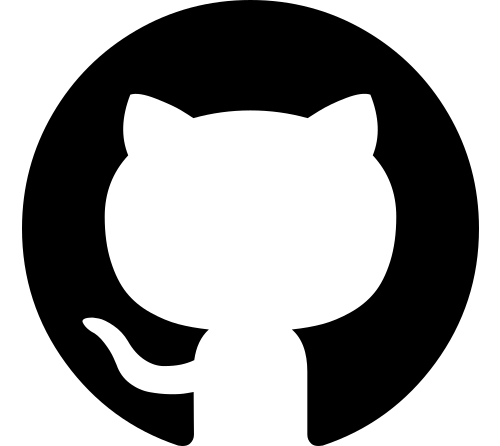
\includegraphics[height=.05\textheight]{resources/github-icon.png}} \includegraphics[height=.05\textheight]{resources/discord-icon.png} ComicSansMS

    \item \href{https://twitter.com/DerGhulbus/}{
\includegraphics[height=.05\textheight]{resources/twitter-icon.png} @DerGhulbus}

    \item 
\includegraphics[height=.05\textheight]{resources/meetup-icon.png} Co-organizer of the \href{https://www.meetup.com/MUCplusplus/}{Munich C++ User Group}

    \item Currently working as a Runtime Engineer for Woven Planet 
\includegraphics[height=.1\textheight]{resources/Woven_Planet_Holdings_Logo.png}

  \end{itemize}
\end{frame}

\begin{frame}[fragile]
  \frametitle{Motivation - File backup}
  
\includegraphics[width=.9\textwidth]{pipelinesgfx/pipe_file_backup_full.png}
\end{frame}

\begin{frame}[fragile]
  \frametitle{Motivation - Media streaming}
  
\includegraphics[width=.9\textwidth]{pipelinesgfx/pipe_media_streaming_full.png}
\end{frame}

\iffalse
\begin{frame}[fragile]
  \frametitle{Motivation}
  \begin{itemize}
    \item Both problems have similarities - Data originating from a source is processed in one or more distinct steps before being handed to sink
    \item Depending on the use case, different requirements for how these individual steps are executed will arise
    \item How can I configure the pipeline to skip and optional step? For instance, if I want to compress, but not encrypt.
  \end{itemize}
\end{frame}
\fi

\begin{frame}
  \frametitle{Motivation - Design Goals}
  
  \begin{itemize}
  \item Be able to implement arbitrary processing steps
  \item Have a unified way to compose steps into a full pipeline
  \item Detailed control about the control flow (i.e. when and how does each step get executed)
  \item Decouple those concerns as much as possible in the implementation, so that they can be changed independently
  \end{itemize}
\end{frame}

\begin{frame}[fragile]
  \frametitle{Motivation - Design Goals}
  \begin{lstlisting}[language={C++}]
FileSource{ from_filename }
  | Compress{}
  | Encrypt{ private_key }
  | NetworkSink{ to_url };
  \end{lstlisting}
\end{frame}

\begin{frame}
  \frametitle{Overview}
  \begin{itemize}
  %\item A taxonomy of processing steps
  \item A general interface for data processing steps
  \item Composing several processing steps into a pipeline
  \item Pipeline control flow
  \item General introduction to coroutines
  \item Coroutines and pipeline control flow
  \end{itemize}
\end{frame}

\begin{frame}

  \frametitle{Warning! Dangerous slide code ahead!}

  \begin{itemize}
    \item The code examples in this presentation are meant to illustrate ideas
    \item They are in no way fit for production and often intentionally omit details like \texttt{const} or \texttt{noexcept} for brevity
    \item Error handling is also frequently missing in code examples
    \item For coroutines I will simplify things and omit details. Check cppreference when implementing your own to understand all the details.
    \item Exercise caution when reimplementing this for production
  \end{itemize}
\end{frame}

\begin{frame}
  \frametitle{Anatomy of a pipeline}
  
  \begin{itemize}
  \item 
\includegraphics[height=.04\textheight]{pipelinesgfx/source.png} Source
  \item 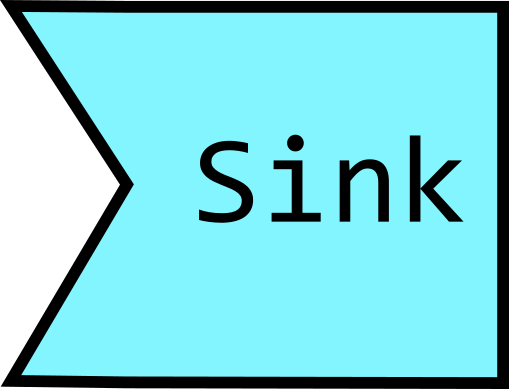
\includegraphics[height=.04\textheight]{pipelinesgfx/sink.png} Sink
  \item 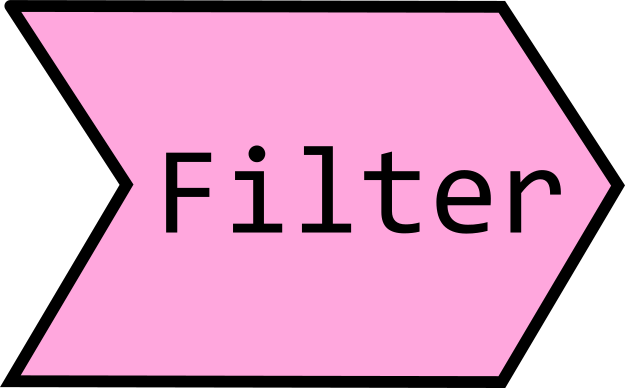
\includegraphics[height=.04\textheight]{pipelinesgfx/filter.png} Filter
  \end{itemize}
  
  \note{Timecheck: 0:05}

\end{frame}

\begin{frame}[fragile]
    \frametitle{A universal interface for processing steps}
    \iftransitions \pause \fi

    \begin{lstlisting}[language={C++}]
zstream zs;
// [...]
zs.next_in = in_buffer;
zs.avail_in = in_buffer_size;
zs.next_out = out_buffer;
zs.avail_out = out_buffer_size;
auto const result = deflate(&zs, Z_NO_FLUSH);
assert(result == Z_OK);
assert((zs.avail_in == 0) || (zs.avail_out == 0));
    \end{lstlisting}
\end{frame}

\begin{frame}
  \frametitle{The zlib interface}
  
  \begin{itemize}
  \item Before each call to deflate, input and output buffers need to be set
  \item A call will process data until either the input is depleted or the output is filled up
  \item Keep calling deflate() in a loop, refilling buffers as needed, until all input has been processed
  \item After all input has been processed, processing enters a finalization phase where all remaining output data is flushed
  \end{itemize}
\end{frame}

\begin{frame}[fragile]
    \frametitle{C++ filter interface}
    
    \begin{lstlisting}[language={C++}]
enum class ProcessReturn { Pending, Done, Error };

struct Filter {
  std::span<std::byte const> in;
  std::span<std::byte> out;
  ProcessReturn process();
};
    \end{lstlisting}
    
    \note{Timecheck: 0:10}
\end{frame}

\begin{frame}[fragile]
    \frametitle{C++ filter interface}
    
    \begin{lstlisting}[language={C++}]
template<typename T>
concept PipelineStage = requires(T a) {
    { a.process() } -> std::same_as<ProcessReturn>;
};
\end{lstlisting}
\iftransitions \pause \fi
\begin{lstlisting}[language={C++}]
template<typename T>
concept PipelineSource = PipelineStage<T> &&
  requires(T a) {
    { a.out } -> std::same_as<std::span<std::byte>&>;
};
    \end{lstlisting}
    \footnote{The \& in \texttt{same\_as} is needed because of \href{https://stackoverflow.com/a/62792349/577603}{https://stackoverflow.com/a/62792349/577603}}
\end{frame}

\begin{frame}[fragile]
  \frametitle{C++ filter interface}

  \begin{lstlisting}[language={C++}]
template<typename T>
concept PipelineSink = PipelineStage<T> &&
  requires(T a) {
    { a.in } ->
       std::same_as<std::span<std::byte const>&>;
};
  \end{lstlisting}
  \iftransitions \pause \fi
  \begin{lstlisting}[language={C++}]
template<typename T>
concept PipelineFilter =
  PipelineSource<T> && PipelineSink<T>;
  \end{lstlisting}
\end{frame}

\iftransitions
\fi

\begin{frame}[fragile]
  \frametitle{Example: File Source \hspace{250pt} 
\includegraphics[height=.1\textheight]{pipelinesgfx/source.png}}
  \begin{lstlisting}[language={C++}]
struct FileSource { FILE* fin; /* ... */ };
FileSource::FileSource(std::string_view fname);

ProcessReturn FileSource::process() { (*@ \iftransitions \pause \fi  @*)
  if (!fin) { return ProcessReturn::Error; }
  if (out.empty()) { return ProcessReturn::Error; } (*@ \iftransitions \pause \fi @*)
  
  std::size_t const bytes_read =
    fread(out.data(), 1, out.size(), fin);
  out = out.subspan(bytes_read);
  
  // ...
  \end{lstlisting}
\end{frame}

\begin{frame}[fragile]
  \frametitle{Example: File Source \hspace{250pt} 
\includegraphics[height=.1\textheight]{pipelinesgfx/source.png}}
  \begin{lstlisting}[language={C++}]
  // ...
  if (feof(fin)) {
      fclose(fin);
      fin = nullptr;
      return ProcessReturn::Done;
  } (*@ \iftransitions \pause \fi @*)
  
  if (ferror(fin)) {
      return ProcessReturn::Error;
  } (*@ \iftransitions \pause \fi @*)
  
  return ProcessReturn::Pending;
}
  \end{lstlisting}
\end{frame}


\begin{frame}[fragile]
  \frametitle{Example: Identity Filter \hspace{230pt} 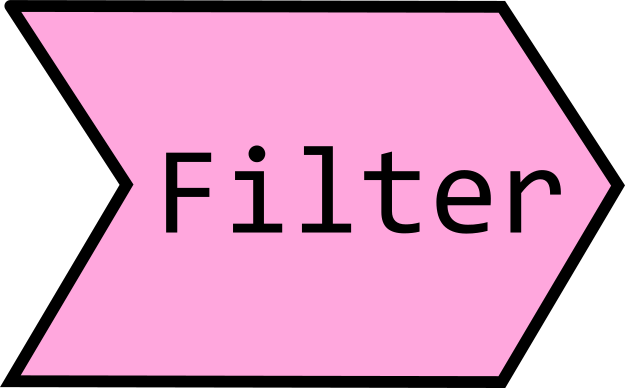
\includegraphics[height=.1\textheight]{pipelinesgfx/filter.png}}
\iftransitions \pause \fi
  \begin{lstlisting}[language={C++}]
ProcessReturn FilterId::process() {
  if (in.empty()) { return ProcessReturn::Done; }
  if (out.empty()) { return ProcessReturn::Error; }  (*@ \iftransitions \pause \fi @*)

  std::size_t const bytes_to_copy =
    std::min(in.size(), out.size());
  std::memcpy(out.data(), in.data(), bytes_to_copy);  (*@ \iftransitions \pause \fi @*)
  in = in.subspan(bytes_to_copy);
  out = out.subspan(bytes_to_copy);

  return ProcessReturn::Pending;
}
  \end{lstlisting}
\end{frame}

\begin{frame}[fragile]
  \frametitle{Example: Deflate Filter \hspace{233pt} 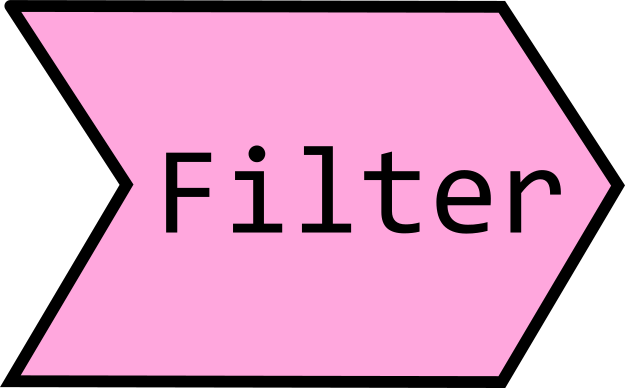
\includegraphics[height=.1\textheight]{pipelinesgfx/filter.png}}
  
  \begin{lstlisting}[language={C++}]
#include <zlib.h>
struct FilterDeflate {
  // ...
  z_stream zs;
};   (*@ \iftransitions \pause \fi @*)
FilterDeflate::FilterDeflate() {
  std::memset(&pimpl->zs, 0, sizeof(z_stream));
  deflateInit(&pimpl->zs, Z_BEST_COMPRESSION);
}    (*@ \iftransitions \pause \fi @*)
FilterDeflate::~FilterDeflate() {
  deflateEnd(&pimpl->zs);
}
  \end{lstlisting}
\end{frame}

\begin{frame}[fragile]
  \frametitle{Example: Deflate Filter \hspace{233pt} 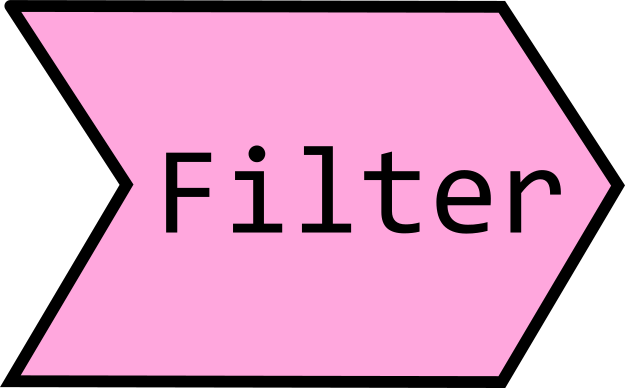
\includegraphics[height=.1\textheight]{pipelinesgfx/filter.png}}
  
  \begin{lstlisting}[language={C++}]
ProcessReturn FilterDeflate::process() {
  bool do_flush = false;  (*@ \iftransitions \pause \fi @*)
  if (zs.avail_in == 0) {
    if (in.empty()) {
      do_flush = true;
    } else {
      zs.next_in =
        reinterpret_cast<Bytef const*>(in.data());
      zs.avail_in = static_cast<uInt>(in.size());
      do_flush = false;
    }
  }
  // ...
  \end{lstlisting}
\end{frame}

\begin{frame}[fragile]
  \frametitle{Example: Deflate Filter \hspace{233pt} 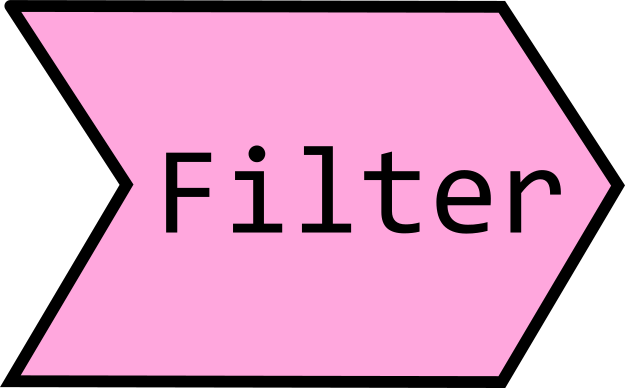
\includegraphics[height=.1\textheight]{pipelinesgfx/filter.png}}
  
  \begin{lstlisting}[language={C++}]
// ...
if (zs.avail_out == 0) {
  if (out.empty()) { return ProcessReturn::Error; }
  zs.next_out = reinterpret_cast<Bytef*>(out.data());
  zs.avail_out = static_cast<uInt>(out.size());
}

// ...
  \end{lstlisting}
\end{frame}

\begin{frame}[fragile]
  \frametitle{Example: Deflate Filter \hspace{233pt} 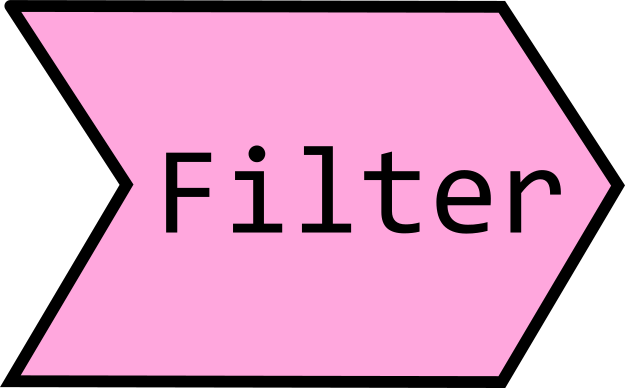
\includegraphics[height=.1\textheight]{pipelinesgfx/filter.png}}
  
  \begin{lstlisting}[language={C++}]
// ...
if (!do_flush) {  (*@ \iftransitions \pause \fi @*)
  auto const res = deflate(&zs, Z_NO_FLUSH);
  if (res != Z_OK) { return ProcessReturn::Error; }  (*@ \iftransitions \pause \fi @*)
  std::size_t in_consumed = in.size() - zs.avail_in;
  in = in.subspan(in_consumed);  (*@ \iftransitions \pause \fi @*)
  std::size_t out_consumed = out.size() - zs.avail_out;
  out = out.subspan(out_consumed);
// ...
  \end{lstlisting}
\end{frame}

\begin{frame}[fragile]
  \frametitle{Example: Deflate Filter \hspace{233pt} 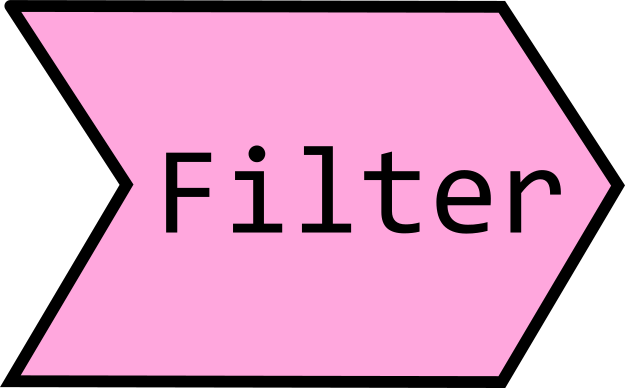
\includegraphics[height=.1\textheight]{pipelinesgfx/filter.png}}
  
  \begin{lstlisting}[language={C++}]
  // ...
  } else /* do_flush */ {
    auto const res = deflate(&zs, Z_FINISH);  (*@ \iftransitions \pause \fi @*)
    if ((res != Z_OK) && (res != Z_STREAM_END))
    { return ProcessReturn::Error; }          (*@ \iftransitions \pause \fi @*)
    out = out.subspan(out.size() - zs.avail_out);  (*@ \iftransitions \pause \fi @*)
    if (res == Z_STREAM_END) {
      deflateReset(&zs);
      return ProcessReturn::Done;
    }
  }  (*@ \iftransitions \pause \fi @*)
  return ProcessReturn::Pending;
}  // process()
  \end{lstlisting}
\end{frame}

\begin{frame}[fragile]
  \frametitle{Connecting multiple stages through buffers}
  
  \iftransitions \pause \fi
  
  \begin{lstlisting}[language={C++}]
class RingBuffer {
public:
  RingBuffer(size_t n_buffers, size_t buffer_size);
  AcquiredBuffer acquireFreeBuffer();
  AcquiredBuffer acquireFilledBuffer();
};
  \end{lstlisting}
  
  \note{Timecheck: 0:20}
\end{frame}

\begin{frame}[fragile]
  \frametitle{Ring Buffer}

  \begin{columns}
    \begin{column}{.5\textwidth}
      \includegraphics<1-2>[width=.95\textwidth]{pipelinesgfx/rbuffer_000.png}
      \includegraphics<3>[width=.95\textwidth]{pipelinesgfx/rbuffer_010.png}
      \includegraphics<4>[width=.95\textwidth]{pipelinesgfx/rbuffer_020.png}
      \includegraphics<5>[width=.95\textwidth]{pipelinesgfx/rbuffer_030.png}
      \includegraphics<6>[width=.95\textwidth]{pipelinesgfx/rbuffer_040.png}
      \includegraphics<7>[width=.95\textwidth]{pipelinesgfx/rbuffer_050.png}
      \includegraphics<8>[width=.95\textwidth]{pipelinesgfx/rbuffer_060.png}
      \includegraphics<9>[width=.95\textwidth]{pipelinesgfx/rbuffer_070.png}
    \end{column}

    \begin{column}{.5\textwidth}
      \begin{semiverbatim}
        \uncover<1->{{RingBuffer b\{ 4, 1024 \};}}
        \uncover<2->{b.acquireFreeBuffer();}
        \uncover<4->{b.acquireFreeBuffer();}
        \uncover<5->{b.acquireFilledBuffer();}
        \uncover<6->{b.acquireFreeBuffer();}
        \uncover<7->{b.acquireFreeBuffer();}
        \uncover<8->{b.acquireFilledBuffer();}
        \uncover<9->{b.acquireFreeBuffer();}
        \uncover<9->{b.acquireFreeBuffer();}
      \end{semiverbatim}
    \end{column}
  \end{columns}
\end{frame}

\begin{frame}[fragile]
  \frametitle{Acquired Buffer Interface}
  
  \begin{lstlisting}[language={C++}]
class AcquiredBuffer {
public:
  AcquiredBuffer(AcquiredBuffer&& rhs) noexcept;
  ~AcquiredBuffer();
  void release();
  void commitBytes(std::size_t n);
  std::span<std::byte> getBuffer() & noexcept;
}; (*@ \iftransitions \pause \fi @*)
{
  AcquiredBuffer acq = b.acquireFreeBuffer();
  size_t const bytes_written = writeTo(acq.getBuffer());
  acq.commitBytes(bytes_written);
}
  \end{lstlisting}
\end{frame}

\begin{frame}
  \frametitle{Connecting steps with buffers}
  \begin{center}
    
\includegraphics[width=.80\textwidth]{pipelinesgfx/pipe_with_buffers.png}
  \end{center}
  \begin{itemize}
  \item A buffer is inserted between any two stages
  \item The buffer is used as output by the stage to its left and as input by the stage to its right.
  \item Any communication from one stage to its neighbours happens through the buffer.
  \end{itemize}
\end{frame}

\begin{frame}[fragile]
  \frametitle{Connecting multiple stages through buffers}
  
  \begin{lstlisting}[language={C++}]
enum class OpState {
  Run, Finalize, Done, Error, Abort
};
  \end{lstlisting} \iftransitions \pause \fi
  
  \begin{lstlisting}[language={C++}]
class RingBuffer {
public:
  RingBuffer(size_t n_buffers, size_t buffer_size);
  AcquiredBuffer acquireFreeBuffer();
  AcquiredBuffer acquireFilledBuffer();
  
  OpState operation_state;
};
  \end{lstlisting}
\end{frame}

\begin{frame}[fragile]
  \frametitle{Pipeline Control Flow}
  
  Recap of what we have so far:
  \begin{itemize}
  \item Source, Sink and Filter
  \begin{lstlisting}[language={C++}]
struct Filter {
  std::span<std::byte> in;
  std::span<std::byte> out;
  ProcessReturn process();
};
  \end{lstlisting}     \iftransitions \pause \fi
  \item RingBuffer
  \begin{lstlisting}[language={C++}]
struct RingBuffer {
  AcquiredBuffer acquireFreeBuffer();
  AcquiredBuffer acquireFilledBuffer();
  OpState operation_state;
};
  \end{lstlisting}
  \end{itemize}
\end{frame}

\begin{frame}[fragile]
  \frametitle{Synchronous Case: Producer-driven}
  
  \begin{center}
\includegraphics<1>[width=.95\textwidth]{pipelinesgfx/pipe_pd_010.png}
\includegraphics<2>[width=.95\textwidth]{pipelinesgfx/pipe_pd_020.png}
\includegraphics<3>[width=.95\textwidth]{pipelinesgfx/pipe_pd_025.png}
\includegraphics<4>[width=.95\textwidth]{pipelinesgfx/pipe_pd_030.png}
\includegraphics<5>[width=.95\textwidth]{pipelinesgfx/pipe_pd_035.png}
\includegraphics<6>[width=.95\textwidth]{pipelinesgfx/pipe_pd_040.png}
  \end{center}

\end{frame}

\begin{frame}[fragile]
  \frametitle{Synchronous Case: Producer-driven \hspace{180pt} 
\includegraphics[height=.1\textheight]{pipelinesgfx/source.png}}

  \begin{lstlisting}[language={C++}]
void executeStep(PipelineSource auto& source,
                 RingBuffer& b_out, auto&& downstream) {  
  while (true) { (*@ \iftransitions \pause \fi @*)
    auto acq = b_out.acquireFreeBuffer();
    source.out = acq.getBuffer();  (*@ \iftransitions \pause \fi @*)
    ProcessReturn ret = source.process();
    if (ret == ProcessReturn::Done) { break; }  (*@ \iftransitions \pause \fi @*)
    size_t const bytes_written =
      acq.getBuffer().size() - source.out.size();
    acq.commitBytes(bytes_written);  (*@ \iftransitions \pause \fi @*)
    downstream();
  }
}
  \end{lstlisting}
\end{frame}

\begin{frame}[fragile]
  \frametitle{Synchronous Case: Producer-driven \hspace{180pt} 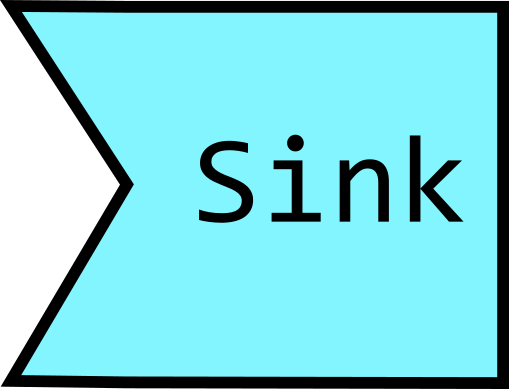
\includegraphics[height=.1\textheight]{pipelinesgfx/sink.png}}

  \begin{lstlisting}[language={C++}]
void executeStep(PipelineSink auto& sink,
                 RingBuffer& b_in) {  (*@ \iftransitions \pause \fi @*)
  auto acq = b_in.acquireFilledBuffer();
  source.in = acq.getBuffer();  (*@ \iftransitions \pause \fi @*)
  ProcessReturn ret = source.process();
  if (ret == ProcessReturn::Done) { return; }
}
  \end{lstlisting}  \iftransitions \pause \fi
  
  \begin{lstlisting}[language={C++}]
executeStep(source, buffer, [&]() {
    executeStep(sink, buffer);
  });
  \end{lstlisting}
\end{frame}

\begin{frame}[fragile]
  \frametitle{Synchronous Case: Producer-driven \hspace{180pt} 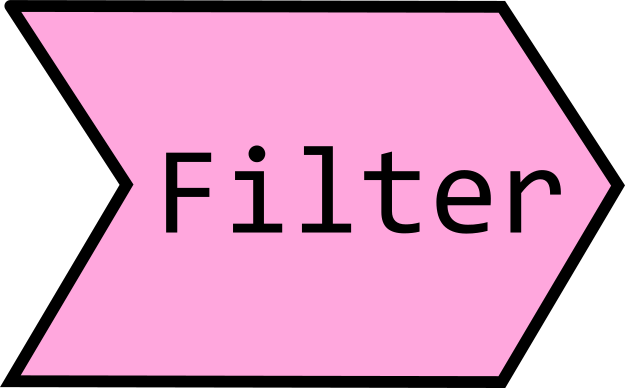
\includegraphics[height=.1\textheight]{pipelinesgfx/filter.png}}

  Just combine source and sink steps?
  
\begin{lstlisting}[language={C++}]
void executeStep(PipelineFilter auto& filter,
                 RingBuffer& b_in,
                 RingBuffer& b_out,
                 auto&& downstream)
\end{lstlisting}  \iftransitions \pause \fi
  \begin{itemize}
  \item Processing may empty either the in buffer, or the out buffer, but not necessarily both  \iftransitions \pause \fi
  \item If the out buffer is not filled, we need to return back to the producer to get another input buffer filled  \iftransitions \pause \fi
  \item But what do we do with the \texttt{AcquiredBuffer} for the output in that case? RAII no longer working nicely.
  \end{itemize}
\iffalse
  \begin{lstlisting}[language={C++}]
void executeStep(PipelineFilter auto& filter,
                 RingBuffer& b_in,
                 RingBuffer& b_out,
                 auto&& downstream) {
  auto acq_in = b_in.acquireFilledBuffer();
  filter.in = acq_in.getBuffer();
  auto acq_out = b_out.acquireFreeBuffer();
  filter.out = acq_out.getBuffer();
  ProcessReturn ret = source.process();
  if (ret != ProcessReturn::Pending) { /* set OpState and return */ }
  if (filter.in.empty()) { /* return to upstream for more input */ return; }
  acq_out.commitBytes( /* ... */ );
  downstream();
}
  \end{lstlisting}
\fi
\end{frame}

\begin{frame}[fragile]
  \frametitle{Synchronous Case: Producer-driven vs. Consumer-driven}

  \includegraphics<1>[width=.9\textwidth]{pipelinesgfx/pipe_pd_000.png}

  \includegraphics<2>[width=.9\textwidth]{pipelinesgfx/pipe_cd_000.png}
\end{frame}

\begin{frame}[fragile]
  \frametitle{Synchronous Case: Producer-driven vs. Consumer-driven}
  
  \begin{lstlisting}[language={C++}]
// producer-driven:
executeStep(source, buffer, [&]() {
    executeStep(sink, buffer);
  });
  \end{lstlisting}

\begin{lstlisting}[language={C++}]
// consumer-driven:
executeStep(sink, buffer, [&]() {
    executeStep(source, buffer);
  });
  \end{lstlisting}
\end{frame}

\begin{frame}[fragile]
  \frametitle{Parallel case}
  
  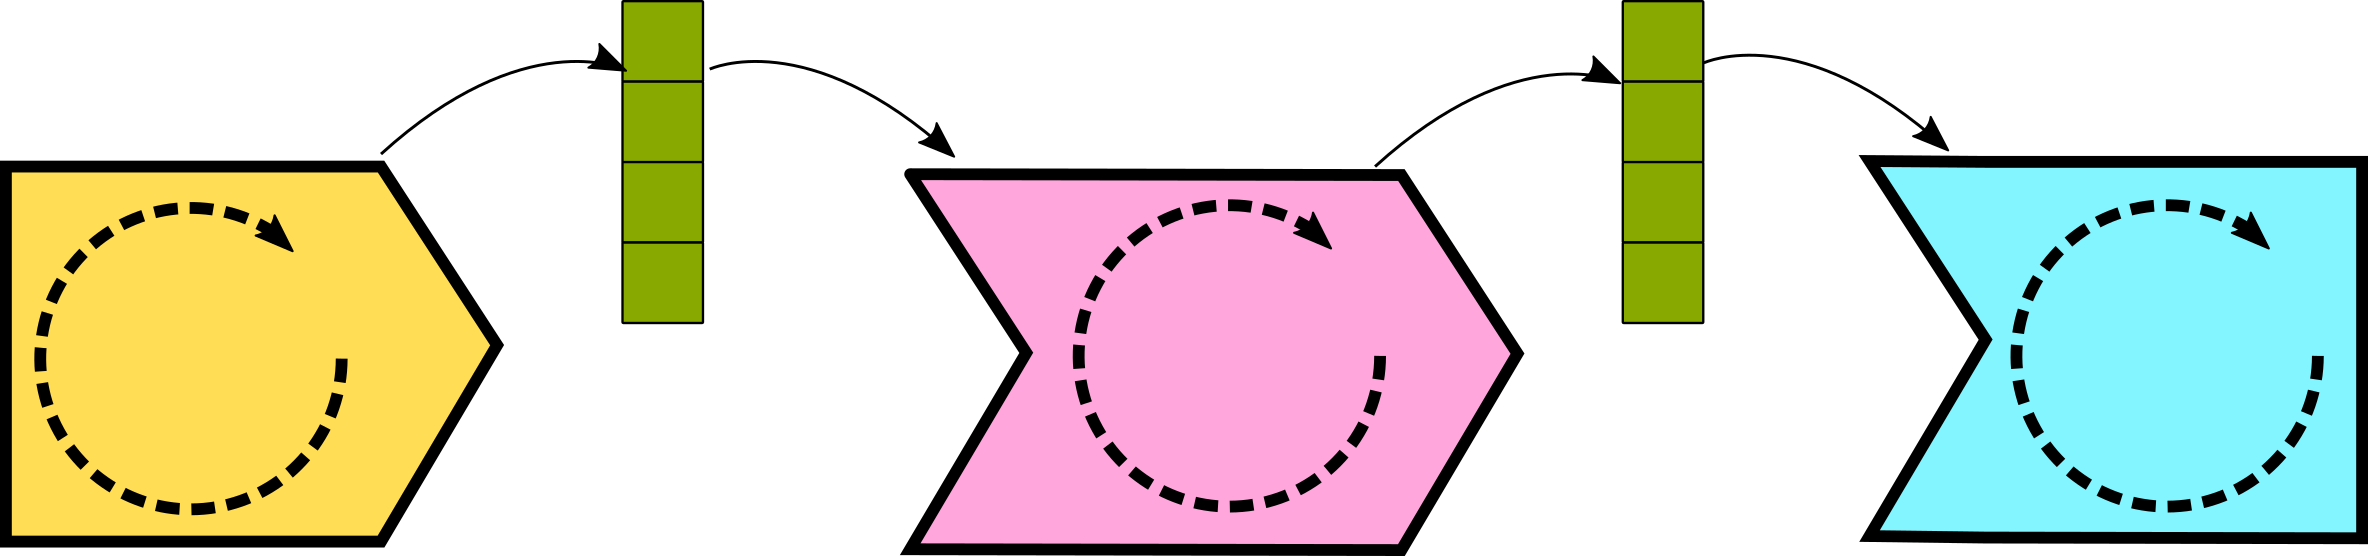
\includegraphics[width=.9\textwidth]{pipelinesgfx/pipe_parallel.png}
  
  Ring buffer is now accessed concurrently!
  
  \note{Timecheck: 0:30}
\end{frame}

\begin{frame}[fragile]
  \frametitle{Thread safe Ring Buffer access}
  
  Single producer, single consumer Ring Buffer

  \begin{lstlisting}[language={C++}]
struct RingBuffer {
  AcquiredBuffer acquireFreeBuffer();
  AcquiredBuffer acquireFilledBuffer();
  OpState operation_state;
};
  \end{lstlisting}
\end{frame}

\begin{frame}[fragile]
  \frametitle{Thread safe Ring Buffer access}
  
  Single producer, single consumer Ring Buffer

  \begin{lstlisting}[language={C++}]
struct MTRingBuffer {
  MTAcquiredBuffer acquireFreeBuffer();
  MTAcquiredBuffer acquireFilledBuffer();
  RingBuffer b_;
};
  \end{lstlisting}
\end{frame}

\begin{frame}[fragile]
  \frametitle{Thread safe Ring Buffer access}

  \begin{lstlisting}[language={C++}]
MTAcquiredBuffer MTRingBuffer::acquireFilledBuffer()
{
  std::unique_lock lk{ mtx };  (*@ \iftransitions \pause \fi @*)
  AcquiredBuffer ret;
  cv.wait(lk, [this, &ret]() -> bool {
    ret = b_.acquireFilledBuffer();
    return static_cast<bool>(ret) ||
      (b_.operation_state() != OpState::Run);
  });  (*@ \iftransitions \pause \fi @*)
  return MTAcquiredBuffer{ this, std::move(ret) };
}
  \end{lstlisting}
\end{frame}


\begin{frame}[fragile]
  \frametitle{Parallel Case \hspace{320pt} 
\includegraphics[height=.1\textheight]{pipelinesgfx/source.png}}

  \begin{lstlisting}[language={C++}]
ProcessReturn executeStep(PipelineSource auto& step,
                  PipelineBuffer auto& out_buffer) { (*@ \iftransitions \pause \fi @*)
  ProcessReturn ret = ProcessReturn::Pending;
  while(ret == ProcessReturn::Pending) { (*@ \iftransitions \pause \fi @*)
    auto acq = out_buffer.acquireFreeBuffer();
    step.out = acquired_buffer.getBuffer();  (*@ \iftransitions \pause \fi @*)
    ret = step.process();
    if (ret != ProcessReturn::Pending) { break; } (*@ \iftransitions \pause \fi @*)
    acq.commitBytes(...);
  }
  return ret;
}
  \end{lstlisting}
\end{frame}

\iffalse
if (ret == ProcessReturn::Done) {
      out_buffer.operation_state = OpState::Finalize;
  }
\fi

\begin{frame}[fragile]
  \frametitle{Parallel Case \hspace{320pt} 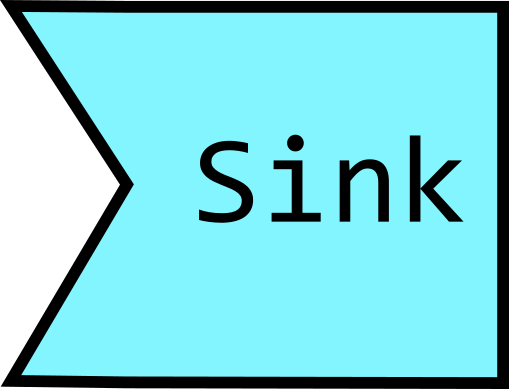
\includegraphics[height=.1\textheight]{pipelinesgfx/sink.png}}

  \begin{lstlisting}[language={C++}]
ProcessReturn executeStep(PipelineSink auto& step,
                 PipelineBuffer auto& in_buffer) { (*@ \iftransitions \pause \fi @*)
  ProcessReturn ret = ProcessReturn::Pending;
  while (ret == ProcessReturn::Pending) { (*@ \iftransitions \pause \fi @*)
    auto acquired_buffer =
      in_buffer.acquireFilledBuffer();
    step.in = acquired_buffer.getBuffer(); (*@ \iftransitions \pause \fi @*)
    ret = step.process();
    if (ret != ProcessReturn::Pending) { break; }
  }
  return ret;
}
  \end{lstlisting}
\end{frame}

\begin{frame}[fragile]
  \frametitle{Parallel Case \hspace{310pt} 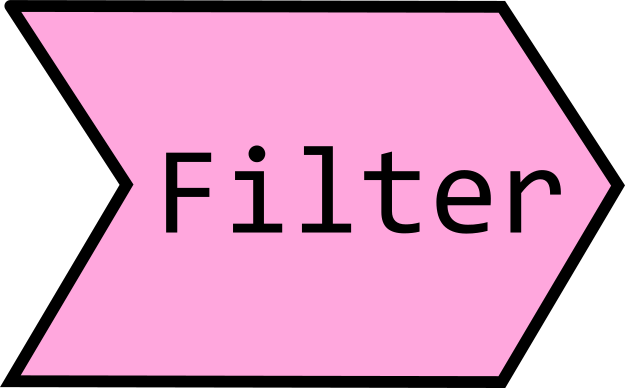
\includegraphics[height=.1\textheight]{pipelinesgfx/filter.png}}

  \begin{lstlisting}[language={C++}]
ProcessReturn executeStep(PipelineFilter auto& step,
                    PipelineBuffer auto& in_buffer,
                    PipelineBuffer auto& out_buffer) { (*@ \iftransitions \pause \fi @*)
  ProcessReturn ret = ProcessReturn::Pending;
  while (ret == ProcessReturn::Pending) { (*@ \iftransitions \pause \fi @*)
    if (step.in.empty()) { /* acquire in */ }
    if (step.out.empty()) { /* acquire out */ } 
    ret = step.process();
    // ...
  }
  return ProcessReturn::Error;
}
  \end{lstlisting}
\end{frame}

\begin{frame}[fragile]
  \frametitle{Parallel Case \hspace{310pt} 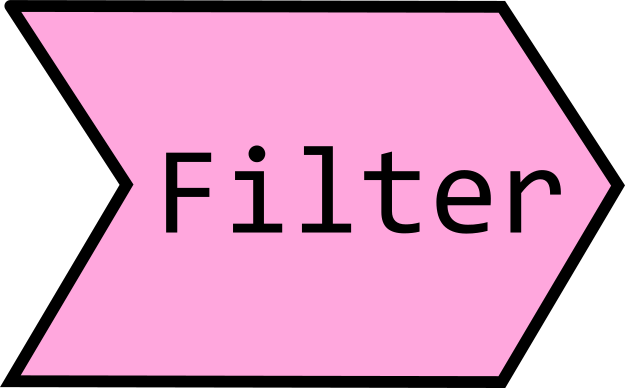
\includegraphics[height=.1\textheight]{pipelinesgfx/filter.png}}

  \begin{lstlisting}[language={C++}]
template<PipelineBuffer InBuffer_T,
         PipelineBuffer OutBuffer_T>
ProcessReturn executeStep(PipelineFilter auto& step,
                          InBuffer_T& in_buffer,
                          OutBuffer_T& out_buffer)
{
    std::optional<typename InBuffer_T::BufferType>
      opt_acquired_in;
    std::optional<typename OutBuffer_T::BufferType>
      opt_acquired_out;
    // ...
}
  \end{lstlisting}
\end{frame}

\begin{frame}[fragile]
  \frametitle{Parallel Case \hspace{310pt} 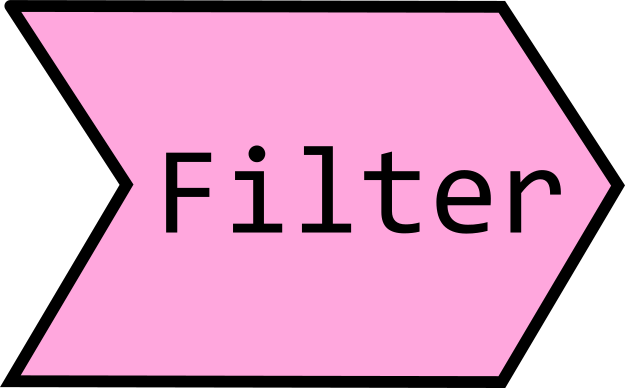
\includegraphics[height=.1\textheight]{pipelinesgfx/filter.png}}

  \begin{lstlisting}[language={C++}]
while (ret == ProcessReturn::Pending) {
  // acquire in
  if (step.in.empty()) {  (*@ \iftransitions \pause \fi @*)
    assert(!opt_acquired_in);
    opt_acquired_in = in_buffer.acquireFilledBuffer();
    step.in = opt_acquired_in->getBuffer();
  }
  // ...  (*@ \iftransitions \pause \fi @*)
  ret = step.process();
  if (step.in.empty()) {
    opt_acquired_in = std::nullopt;
  }
}
  \end{lstlisting}
\end{frame}


\begin{frame}[fragile]
  \frametitle{Parallel Case \hspace{310pt} 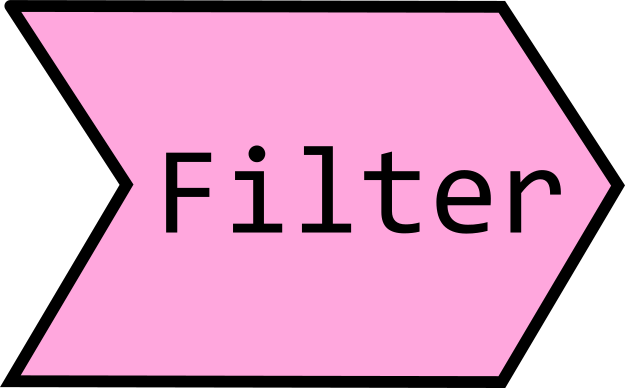
\includegraphics[height=.1\textheight]{pipelinesgfx/filter.png}}

  \begin{lstlisting}[language={C++}]
while (ret == ProcessReturn::Pending) {
  // ...
  // acquire out
  if (step.out.empty()) {
    opt_acquired_out = out_buffer.acquireFreeBuffer();;
    step.out = opt_acquired_out->getBuffer();
  }
  ret = step.process();
  // ...  (*@ \iftransitions \pause \fi @*)
  if (step.out.empty()) {
    opt_acquired_out->commitBytes(size);
    opt_acquired_out = std::nullopt;
  }
  \end{lstlisting}
\end{frame}

\begin{frame}[fragile]

\frametitle{Parallel Case - User View}

\begin{lstlisting}[language={C++}]
FileSource source{ fname_src };
FileSink sink{ fname_dst };
FilterDeflate deflate;
MTRingBuffer b1, b2;
std::jthread t1{ [&] { executeStep(source, b1); } };
std::jthread t2{ [&] { executeStep(deflate, b1, b2); } };
std::jthread t3{ [&] { executeStep(sink, b2); } };
\end{lstlisting}

\end{frame}

\begin{frame}

  \frametitle{Recap: Control Flow}
  
  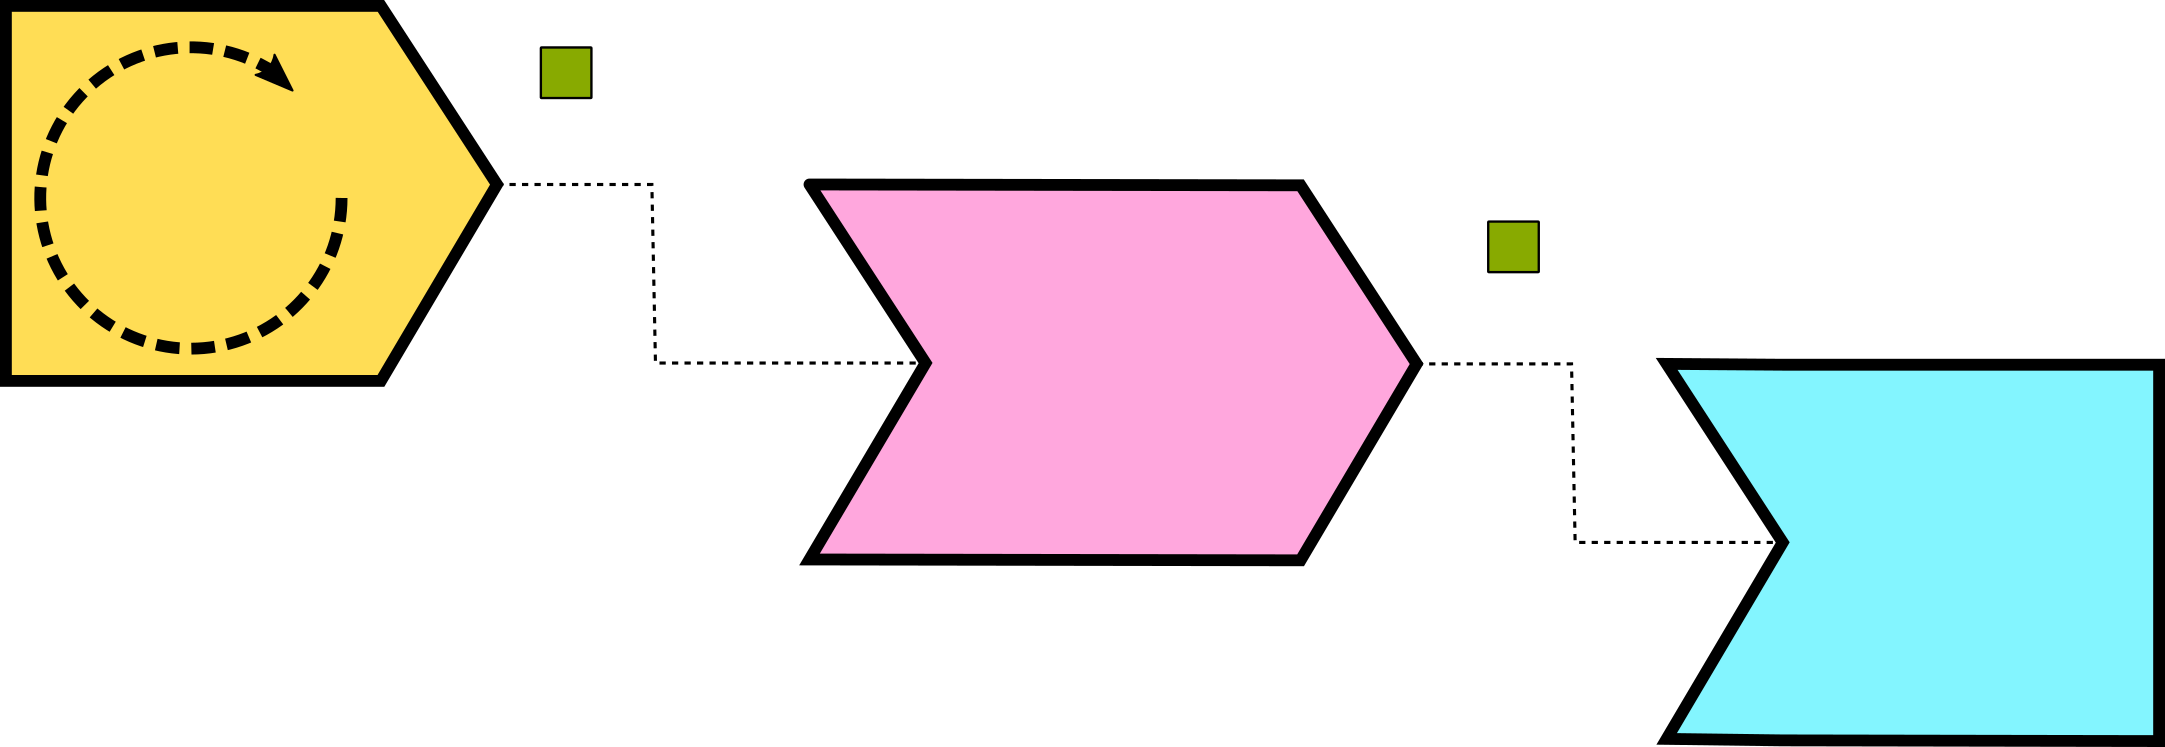
\includegraphics[height=.25\textheight]{pipelinesgfx/pipe_pd_000.png} \hfill
  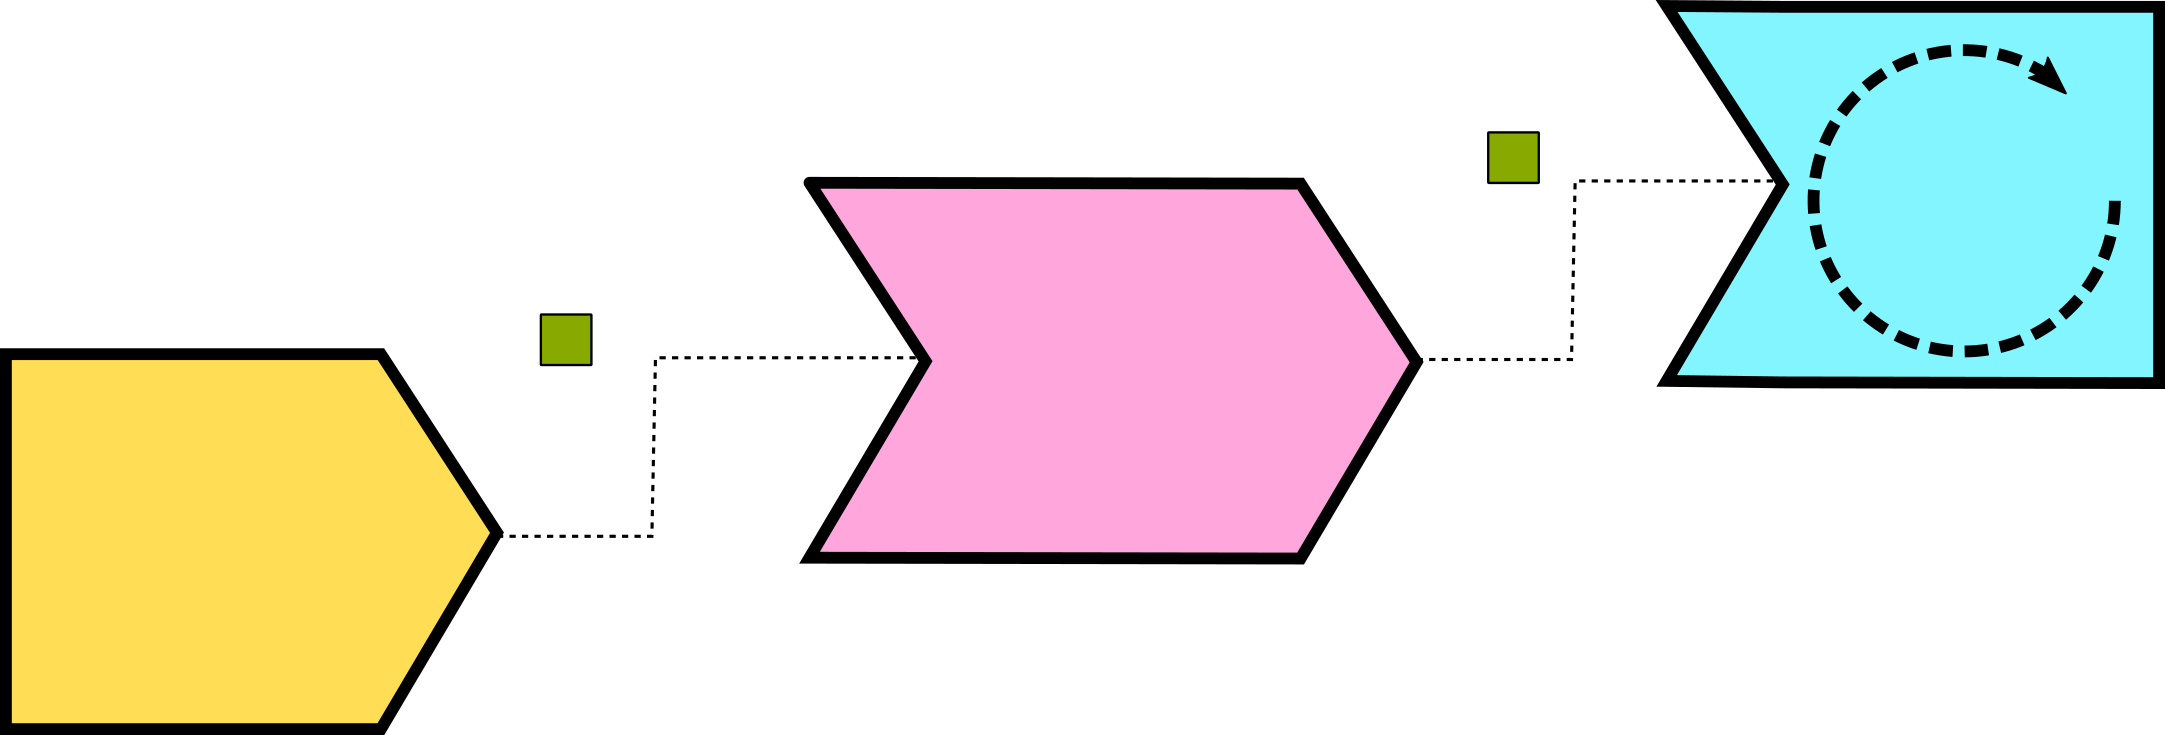
\includegraphics[height=.25\textheight]{pipelinesgfx/pipe_cd_000.png}
  
  \vspace{10pt}
  
  \begin{center}
  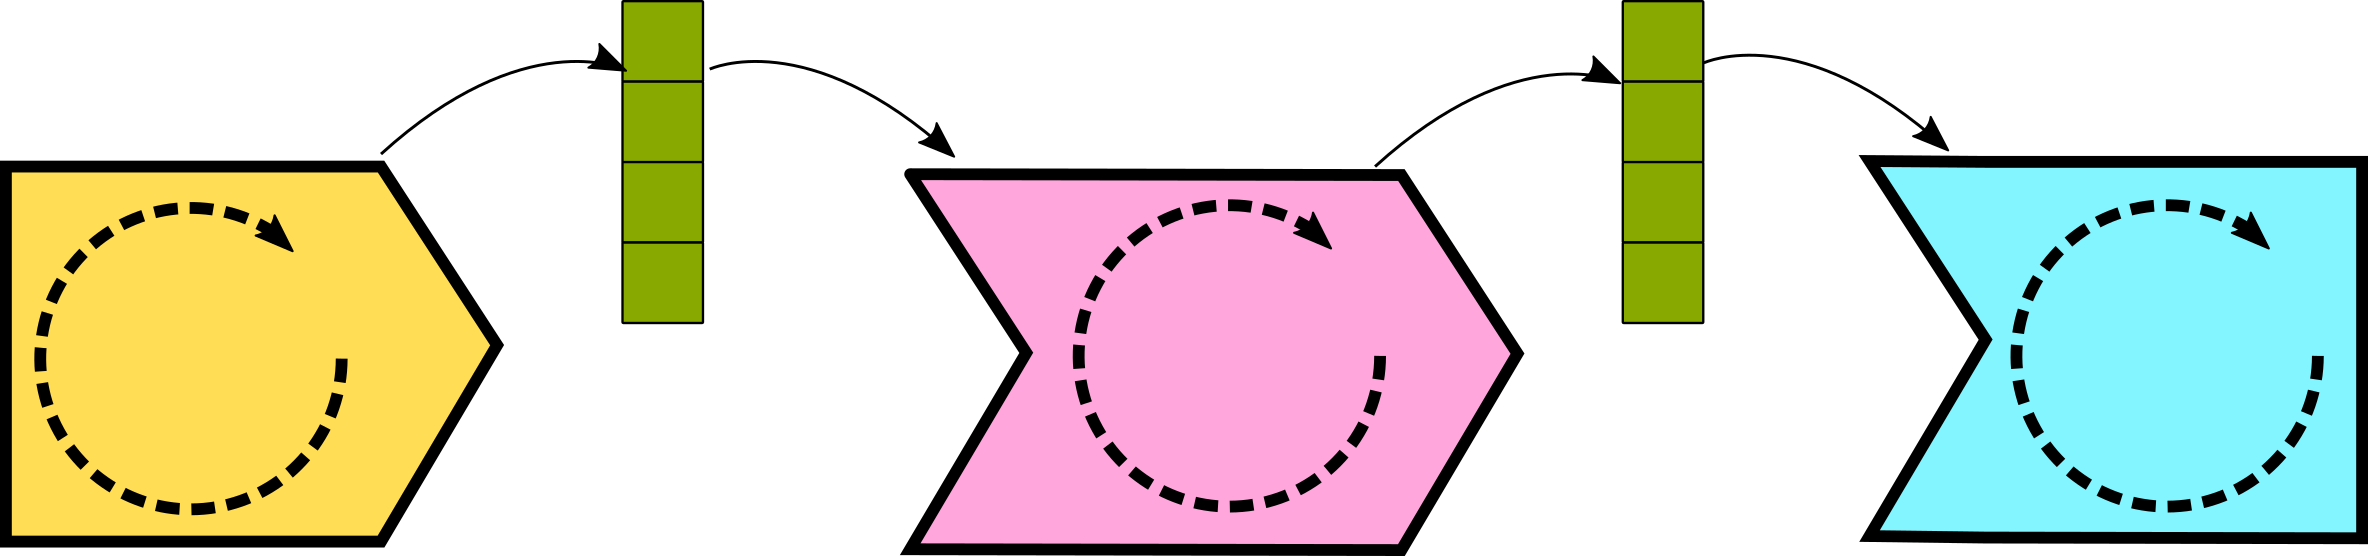
\includegraphics[height=.25\textheight]{pipelinesgfx/pipe_parallel.png}
  \end{center}
\end{frame}

\begin{frame}
    \frametitle{Coroutine Basics}
    
    \begin{itemize}
    \item Coroutines are like a function that can be paused in the middle
    \item Execution can be suspended and resumed later with all surrounding function state still intact
    \item C++ provides stackless coroutines - suspension only affects the currently executing function, but not its parents
    \end{itemize}
    
    \note{Timecheck: 0:40}
\end{frame}

\iffalse
\begin{frame}
    \frametitle{Typical coroutine execution pattern}

    \begin{itemize}
    \item Coroutine \texttt{c()} is invoked from its parent \texttt{main()}.
    \item \texttt{c()} performs some computation and eventually suspends execution.
    \item Control flow returns to \texttt{main()}, potentially yielding a value from \texttt{c()}
    \item At some later point \texttt{c()} gets resumed, potentially this time from a different parent \texttt{p2()}.
    \item \texttt{c()} may continue yielding values indefinitely or eventually complete execution with a final return value.
    \end{itemize}
\end{frame}
\fi

\begin{frame}
    \frametitle{Coroutine Basics - User View}
    
    A coroutine is a function containing either
    \begin{itemize}
    \item \texttt{co\_await}
    \item \texttt{co\_return}
    \item \texttt{co\_yield}
    \end{itemize}
\end{frame}

\begin{frame}[fragile]
  \frametitle{Coroutine Basics - Asynchronous computation}

  \begin{lstlisting}[language={C++}]
auto [ec, bytes_read] = read(socket, buffer);
// ...

async_read(socket, buffer,
  [](std::error_code ec, std::size_t bytes_read) {
    // ...
  });
  \end{lstlisting}
\end{frame}

\begin{frame}[fragile]
  \frametitle{Coroutine Basics - Asynchronous computation}

  \begin{lstlisting}[language={C++}]
auto [ec, bytes_read] = read(socket, buffer);
// ...

auto [ec, bytes_read] =
         co_await async_read(socket, buffer);
// ...
  \end{lstlisting}
\end{frame}


\begin{frame}[fragile]
  \frametitle{Coroutine Basics - Suspend/resume}

  \begin{lstlisting}[language={C++}]
MyCoroutine co = startComputation(initial_data);
auto some_results = co.provide(some_data);
auto more_results = co.provide(more_data);
auto final_results = co.results;
  \end{lstlisting}
\end{frame}

\begin{frame}
  \frametitle{Participants in coroutine execution}
  
  \begin{itemize}
  \item Return object
  \item Promise
  \item Awaitable
  \end{itemize}
\end{frame}

\begin{frame}[fragile]
  \frametitle{Return object}

  \begin{lstlisting}[language={C++}]
MyCoroutine co = startComputation(initial_data);
  \end{lstlisting}

  \begin{itemize}
    \item Return type of the coroutine function   \iftransitions \pause \fi
    \item Typically receives the \texttt{coroutine\_handle} of the started coroutine as constructor argument  \iftransitions \pause \fi
    \item Points out the promise through the nested \texttt{promise\_type} typedef
  \end{itemize}
\end{frame}

\begin{frame}[fragile]
  \frametitle{Promise Type}

  \begin{itemize}
    \item Main point of interaction from within the coroutine  \iftransitions \pause \fi
    \item Constructed by the compiler at the start of the coroutine. Receives initial function arguments as constructor arguments \iftransitions \pause \fi
    \item Determines what happens at essential points in a coroutines' lifetime: Start and completion of execution, exit via \texttt{co\_return} or exception \iftransitions \pause \fi
    \item Responsible for construction of return object through \texttt{get\_return\_object} (needs to be compatible but not same as return object type) \iftransitions \pause \fi
    \item Provides access to \texttt{coroutine\_handle} via \texttt{coroutine\_handle<Promise\_T>::from\_promise()} \iftransitions \pause \fi
    \item Also, promise can be retrieved from the handle via \texttt{promise()} member function on \texttt{coroutine\_handle}
  \end{itemize}
\end{frame}

\begin{frame}[fragile]
  \frametitle{Awaitable}
  
  \begin{lstlisting}[language={C++}]
AsyncRead awaitable = async_read(socket, buffer);
auto [ec, bytes_read] = co_await awaitable;
  \end{lstlisting}

  
  \begin{itemize}
  \item A type that can be \texttt{co\_await}ed on.  \iftransitions \pause \fi
  \item Provides hooks to inject code into the suspend and resume procedures  \iftransitions \pause \fi
  \item May decide not to suspend at all \iftransitions \pause \fi
  \item Gets passed a handle to the running coroutine before suspension.
  \end{itemize}
\end{frame}

\begin{frame}[fragile]
  \frametitle{Minimum boilerplate}
  
  \begin{lstlisting}[language={C++}]
struct Coroutine {
  struct promise_type { /* ... */ };
};

Coroutine f1() {
  co_return;
}

int main() {
  Coroutine c1 = f1();
}
  \end{lstlisting}
\end{frame}

\begin{frame}[fragile]
  \frametitle{Minimum boilerplate}
  
  \begin{lstlisting}[language={C++}]
struct promise_type {
  Coroutine get_return_object();
  std::suspend_never initial_suspend();
  std::suspend_always final_suspend();
  void return_void();
  void unhandled_exception();
};
  \end{lstlisting}
\end{frame}

\begin{frame}[fragile]
  \frametitle{Minimum boilerplate}
  
  \begin{lstlisting}[language={C++}]
Coroutine f1(T... args) {
  // using promise = Coroutine::promise_type;
  // promise __p(args...);
  // __p.get_return_object(); -> to caller
  // co_await __p.initial_suspend()
}

int main() {
  Coroutine c1 = f1();
}
  \end{lstlisting}
\end{frame}

\begin{frame}[fragile]
  \frametitle{Minimum boilerplate}
  
  \begin{lstlisting}[language={C++}]
Coroutine f1(T... args) {
  co_return;
  // __p.return_void();
  // co_await __p.final_suspend()
  // __p.~promise();
}

int main() {
  Coroutine c1 = f1();
}
  \end{lstlisting}
\end{frame}

\begin{frame}[fragile]
  \frametitle{Suspension}
  
  \begin{lstlisting}[language={C++}]
struct MyAwaitable {
  bool await_ready() { return false; }
  void await_suspend(std::coroutine_handle<> h) {}
  void await_resume() {}
};

Coroutine f1(T... args) {
  co_await MyAwaitable{};
  fmt::print("Never reached\n");
}
  \end{lstlisting}
  
  \note{Timecheck: 0:55}
\end{frame}

\begin{frame}[fragile]
  \frametitle{Making acquainances}
  
  \begin{center}
  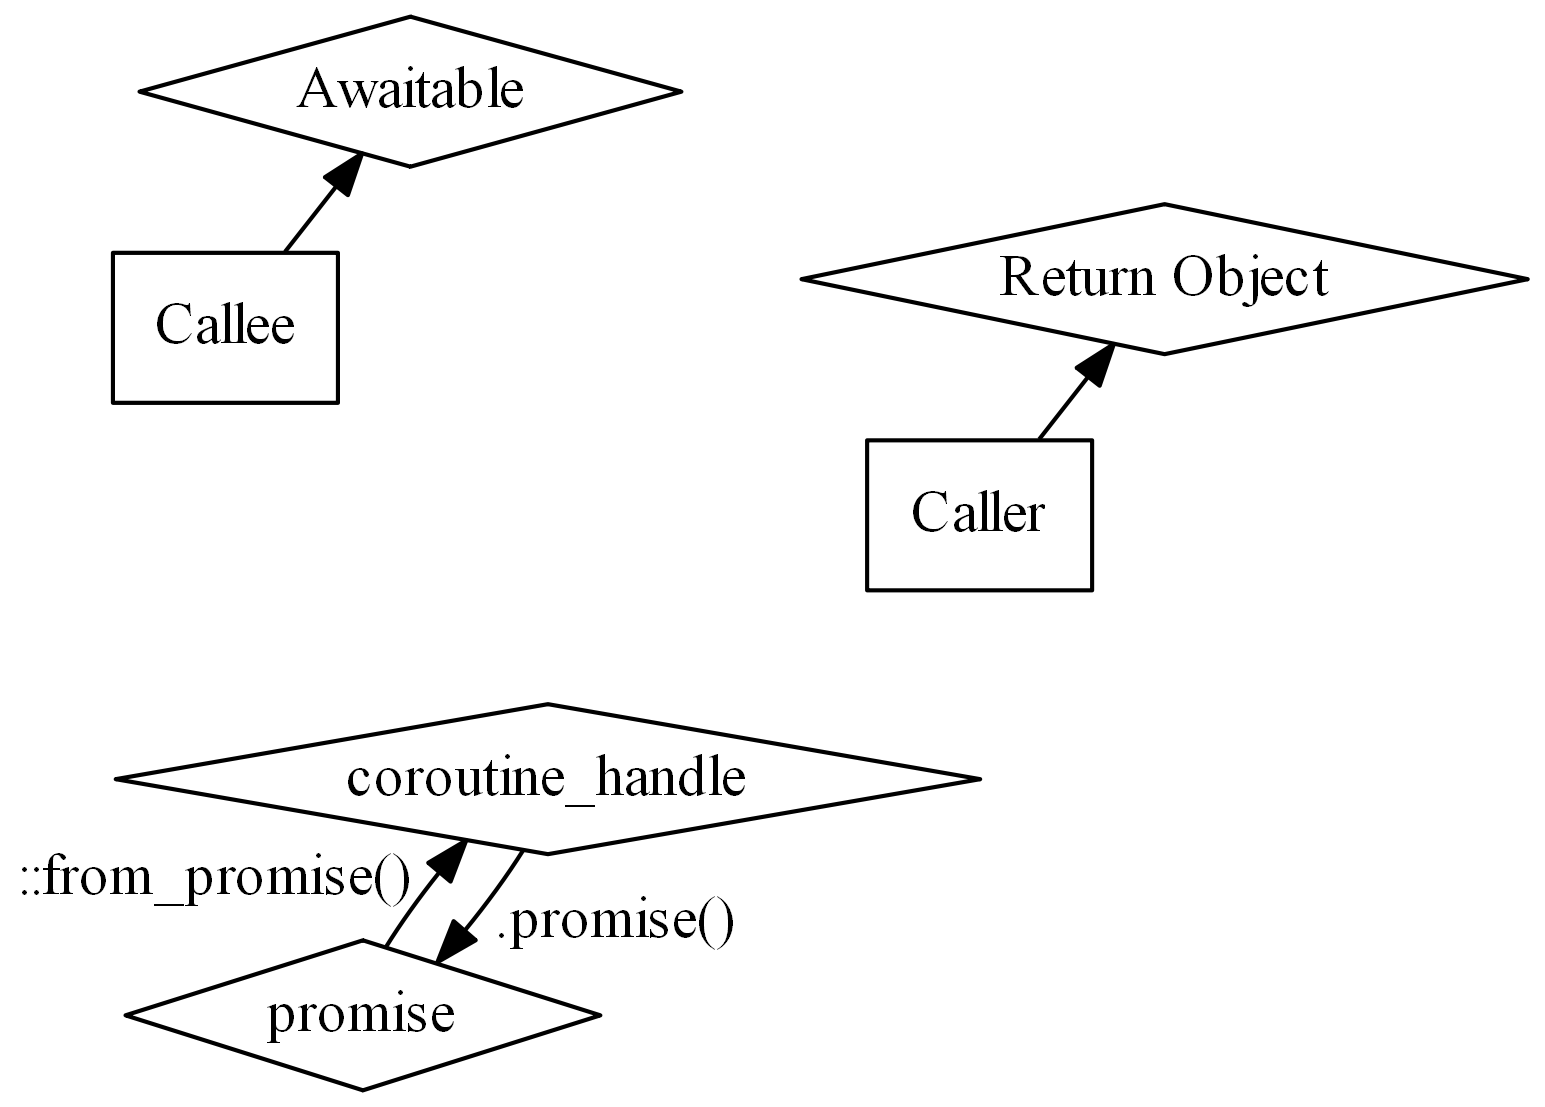
\includegraphics[height=.9\textheight]{pipelinesgfx/acquaintances01.png}
  \end{center}
\end{frame}

\begin{frame}[fragile]
  \frametitle{Making acquainances}

  \begin{lstlisting}[language={C++}]
struct Coroutine {
  std::coroutine_handle<promise_type> handle;
  Coroutine(std::coroutine_handle<promise_type> h)
  : handle(h) {}
};  (*@ \iftransitions \pause \fi @*)
struct promise_type {
  coroutine get_return_object() {
    return coroutine{
      std::coroutine_handle<promise>::from_promise(*this)
      };
  }
};
  \end{lstlisting}
\end{frame}

\begin{frame}[fragile]
  \frametitle{Making acquainances}
  
  \begin{center}
  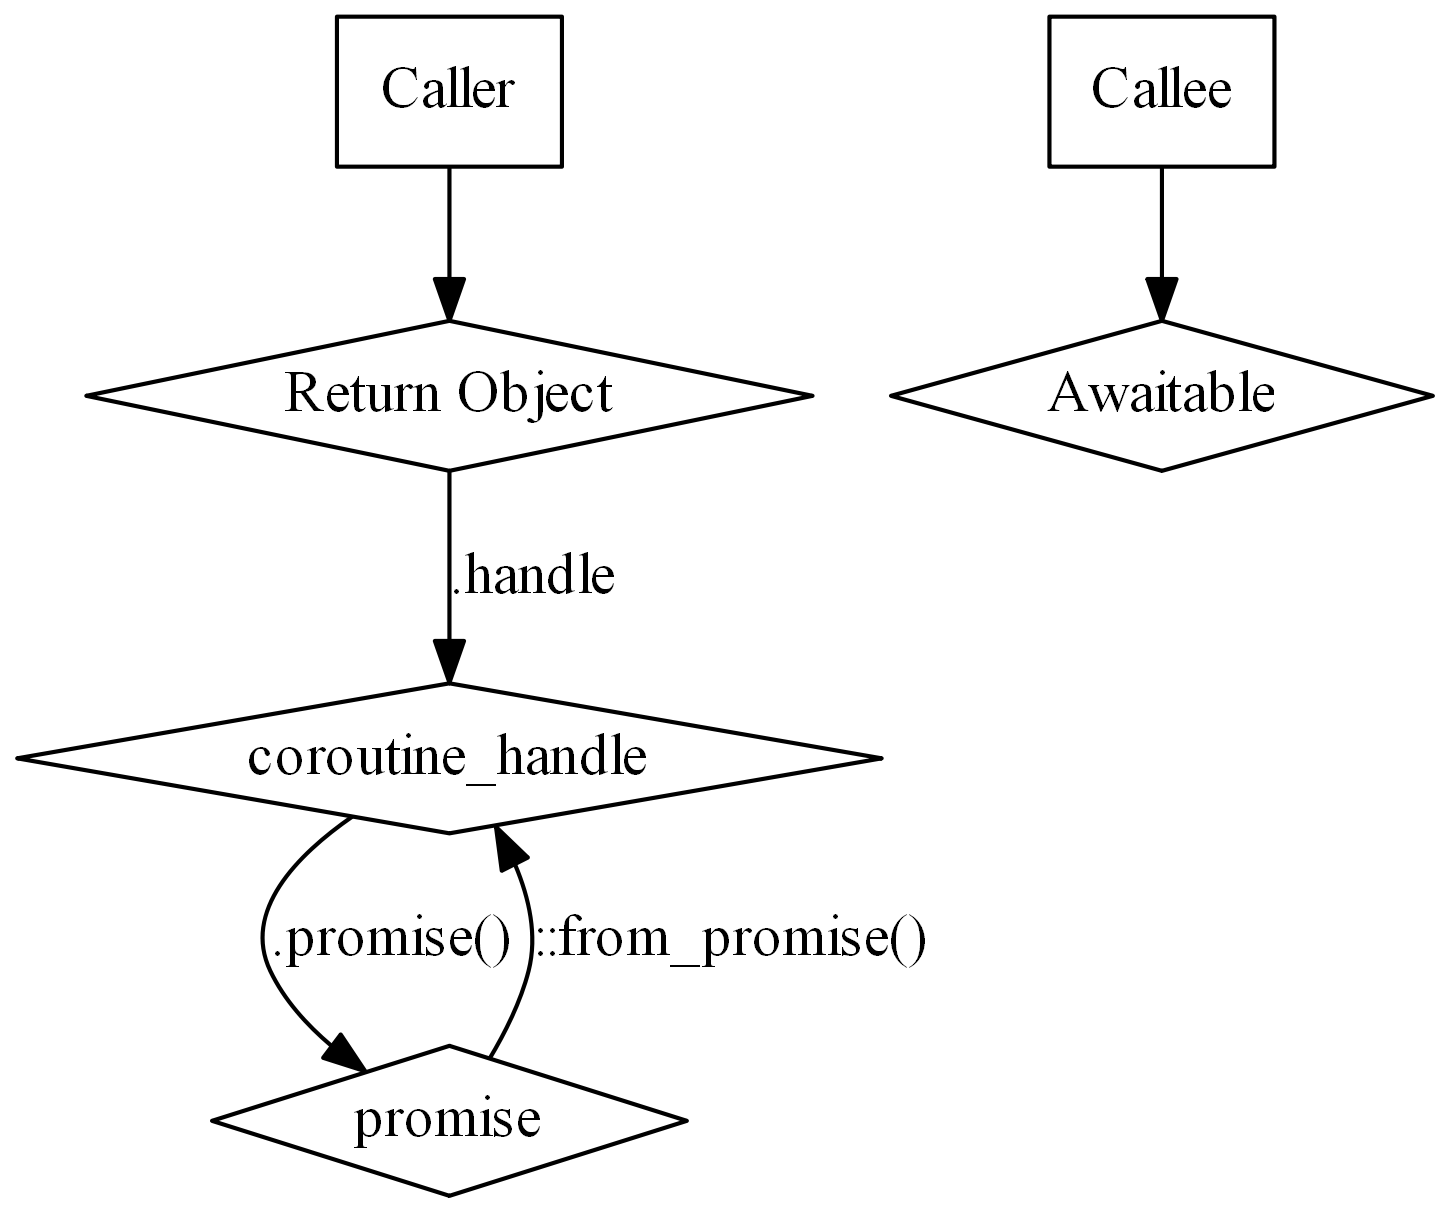
\includegraphics[height=.9\textheight]{pipelinesgfx/acquaintances02.png}
  \end{center}
\end{frame}


\begin{frame}[fragile]
  \frametitle{Making acquainances}

  \begin{lstlisting}[language={C++}]
struct MyAwaitable {
  void await_suspend(std::coroutine_handle<> h) {}
};
  \end{lstlisting}
\end{frame}

\begin{frame}[fragile]
  \frametitle{Our (Incomplete) Map of Coroutine Land}
  
  \begin{center}
  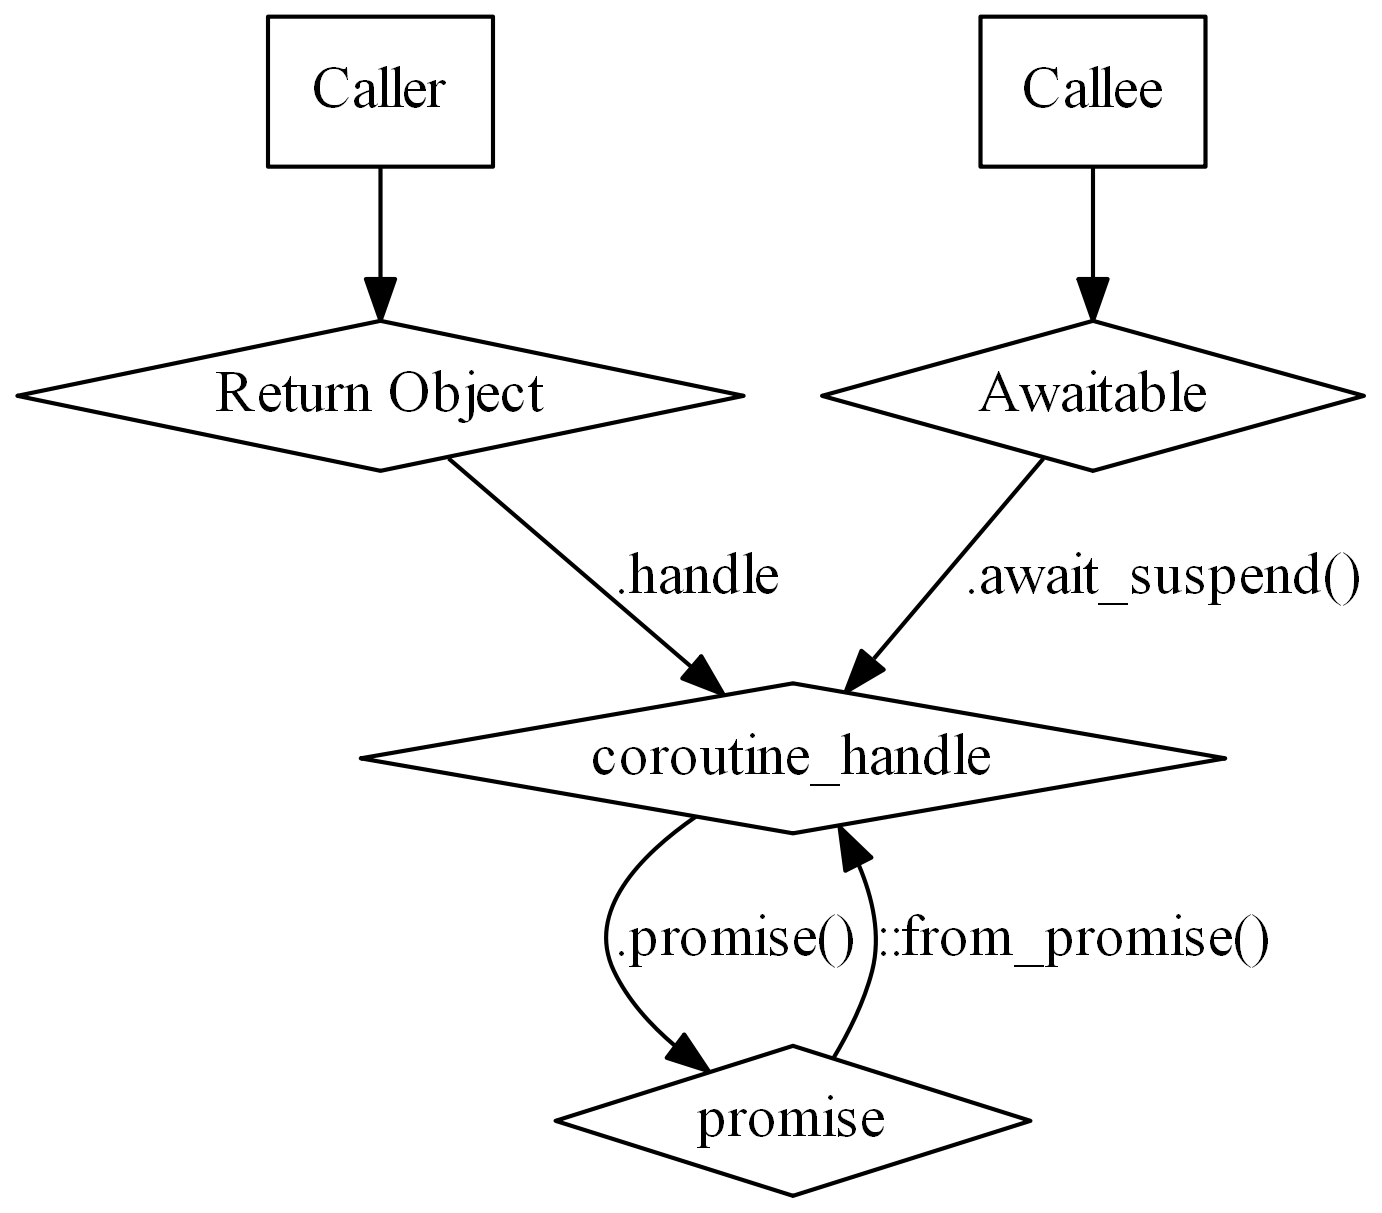
\includegraphics[height=.9\textheight]{pipelinesgfx/acquaintances03.png}
  \end{center}
\end{frame}

\begin{frame}[fragile]
  \frametitle{Getting data out of a coroutine}
  \pause
  \begin{center}
  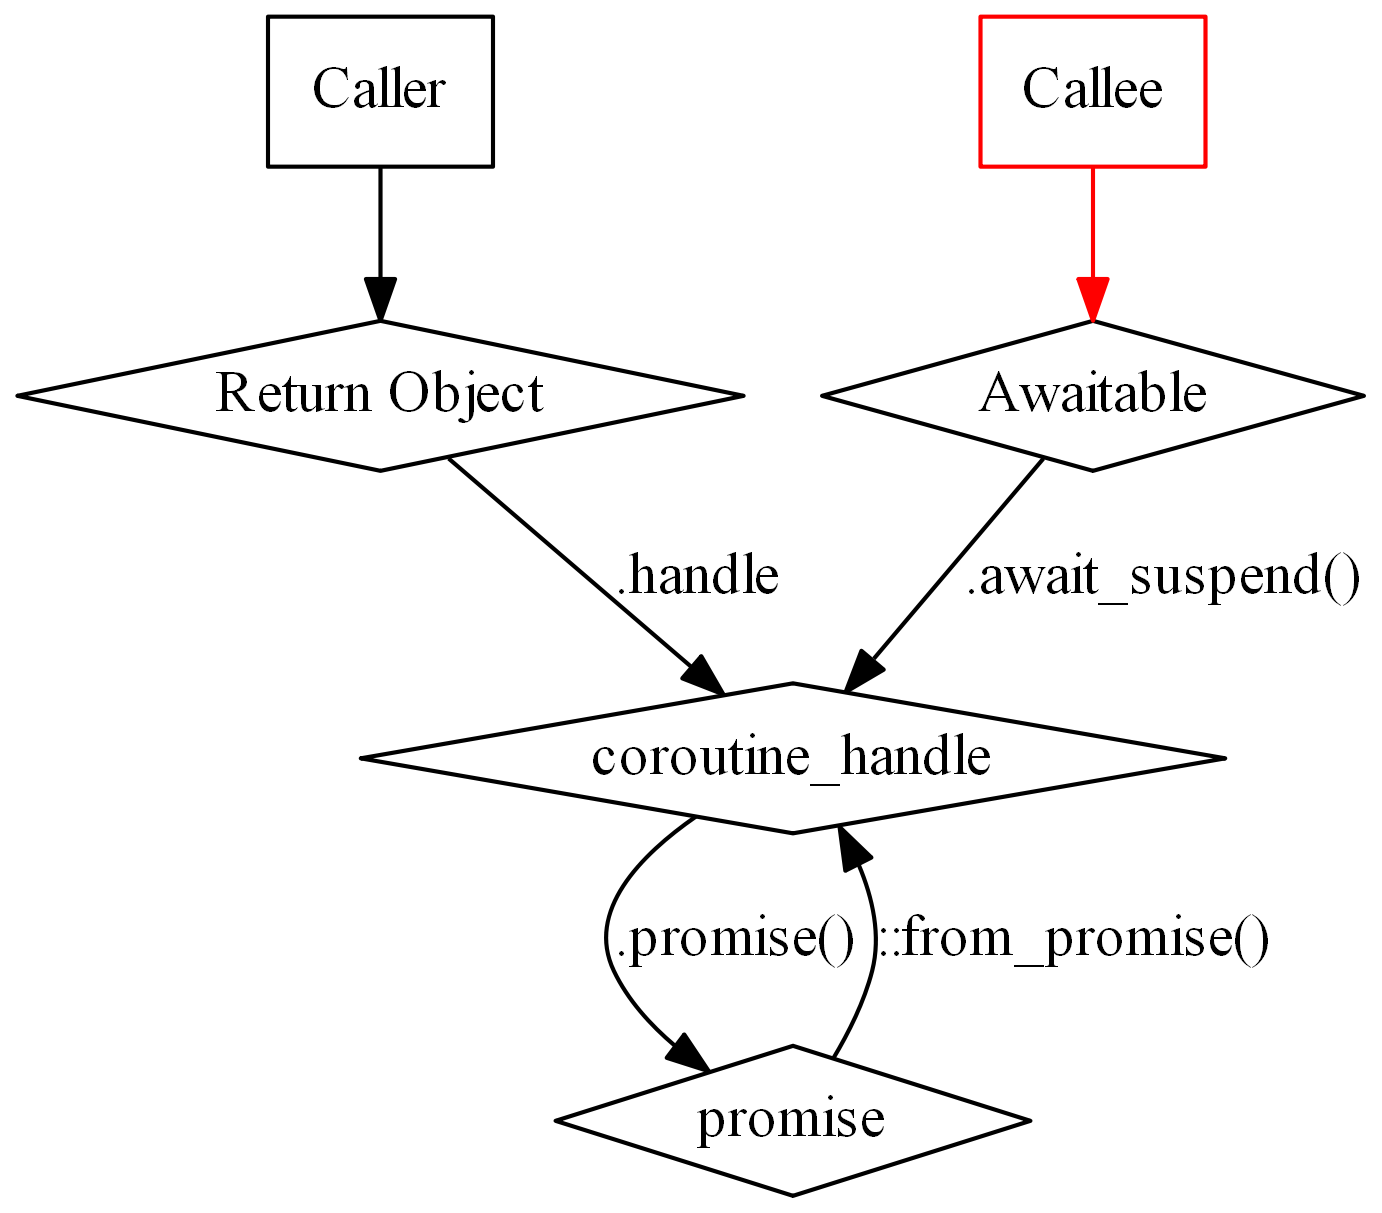
\includegraphics[height=.9\textheight]{pipelinesgfx/path_out_010.png}
  \end{center}
  
  \note{Timecheck: 1:00}
\end{frame}

\begin{frame}[fragile]
  \frametitle{Getting data out of a coroutine}
  
  \begin{lstlisting}[language={C++}]
Coroutine f1() {
  co_await TheAnswer{42};
}

TheAnswer::TheAnswer(int v)
:value_(v) {}
  \end{lstlisting}
\end{frame}

\begin{frame}[fragile]
  \frametitle{Getting data out of a coroutine}

  \begin{center}
  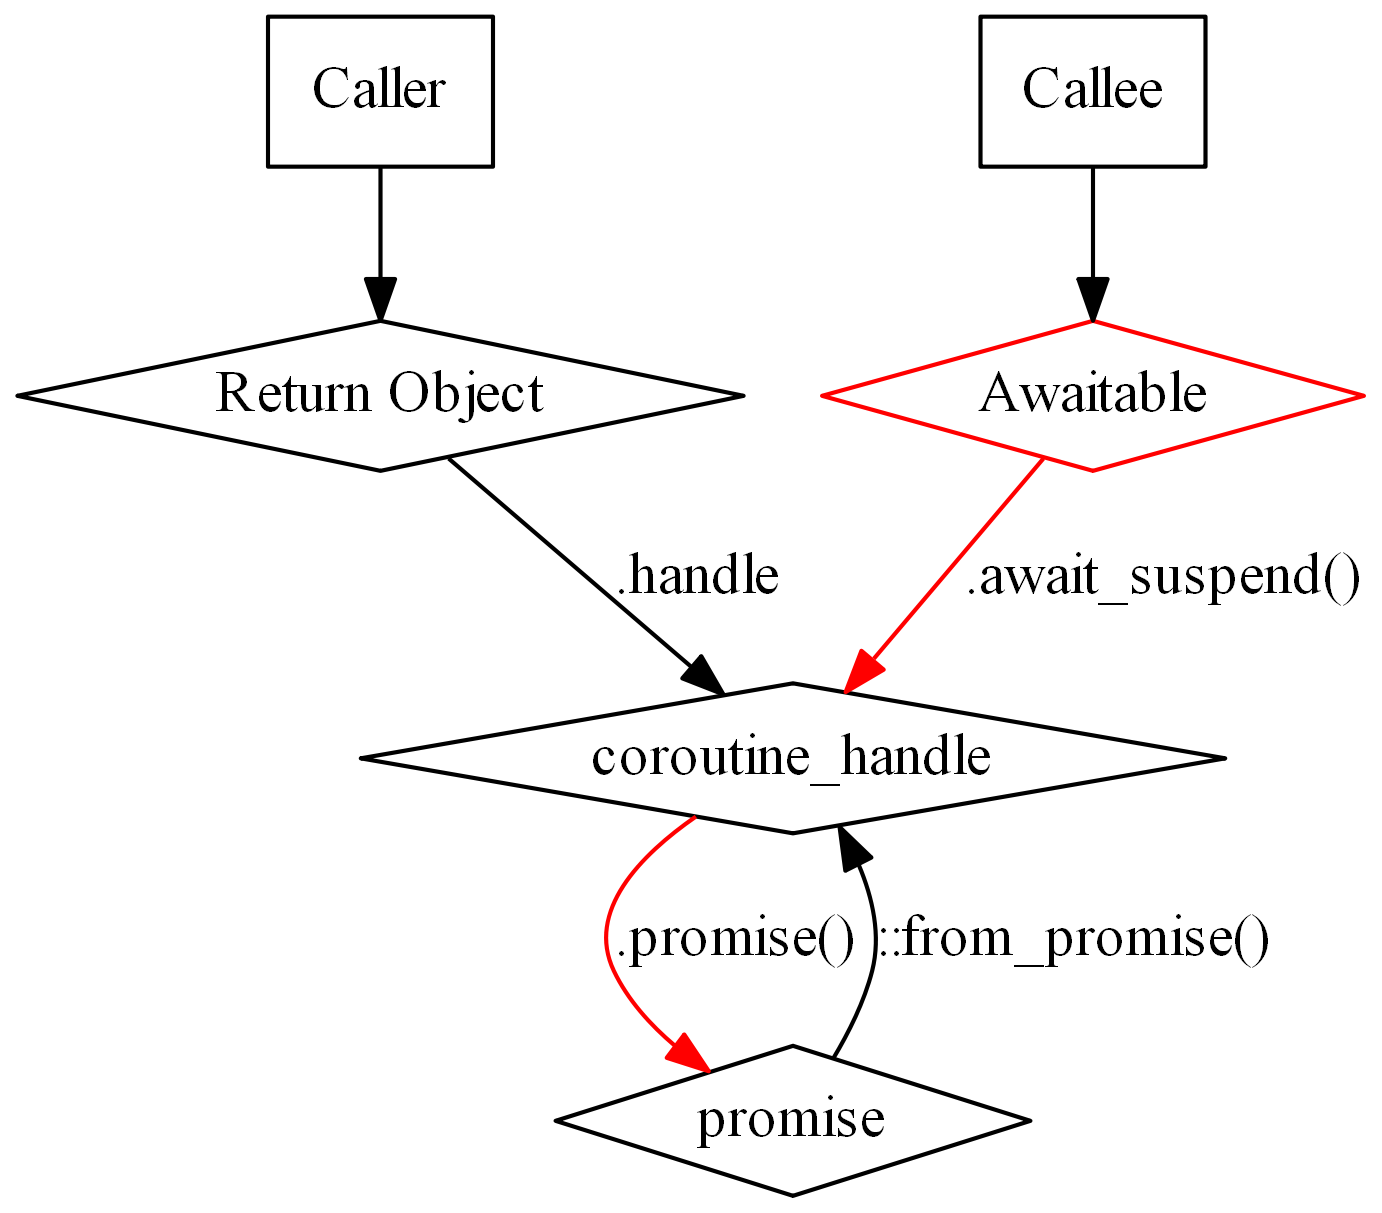
\includegraphics[height=.9\textheight]{pipelinesgfx/path_out_020.png}
  \end{center}
\end{frame}

\begin{frame}[fragile]
  \frametitle{Getting data out of a coroutine}
  
  \begin{lstlisting}[language={C++}]
struct promise {
  // ...
  int value;
};

void TheAnswer::await_suspend(
       std::coroutine_handle<promise> h)
{
  h.to_promise().value = value_;
}
  \end{lstlisting}
\end{frame}

\begin{frame}[fragile]
  \frametitle{Getting data out of a coroutine}

  \begin{center}
  \includegraphics<1>[height=.9\textheight]{pipelinesgfx/path_out_030.png}
  \includegraphics<2>[height=.9\textheight]{pipelinesgfx/path_out_040.png}
  \end{center}
\end{frame}

\iftransitions
\begin{frame}[fragile]
  \frametitle{Getting data out of a coroutine}
  
  \begin{lstlisting}[language={C++}]
struct Coroutine {
  // ...
  
  
  
  
};
int main() {
  Coroutine c1 = f1();
  fmt::print("The answer is {}\n", c1.getAnswer());
}
  \end{lstlisting}
\end{frame} 
\fi

\begin{frame}[fragile]
  \frametitle{Getting data out of a coroutine}
  
  \begin{lstlisting}[language={C++}]
struct Coroutine {
  // ...
  std::coroutine_handle<promise> handle;
  int getAnswer() {
    return handle.promise().value;
  }
};
int main() {
  Coroutine c1 = f1();
  fmt::print("The answer is {}\n", c1.getAnswer());
}
  \end{lstlisting}
\end{frame} 

\begin{frame}
  \frametitle{Getting data into a coroutine}
  
  \begin{center}
  \includegraphics<2>[height=.9\textheight]{pipelinesgfx/path_in_010.png}
  \end{center}
  
  \note{Timecheck: 1:10}
\end{frame}

\begin{frame}[fragile]
  \frametitle{Getting data out of a coroutine}
  
  \begin{lstlisting}[language={C++}]
Coroutine f1() {
  int the_answer = co_await OutsideAnswer{};
}

int main() {
  Coroutine c1 = f1();
  c1.provide(42);
}
  \end{lstlisting}
\end{frame}

\begin{frame}[fragile]
  \frametitle{Getting data out of a coroutine}
  
  \begin{lstlisting}[language={C++}]
void Coroutine::provide(int the_answer) {
  handle.promise().value = the_answer;
  handle.resume();
}
  \end{lstlisting}
\end{frame}

\begin{frame}
  \frametitle{Getting data into a coroutine}
  
  \begin{center}
  \includegraphics<1>[height=.9\textheight]{pipelinesgfx/path_in_020.png}
  \includegraphics<2>[height=.9\textheight]{pipelinesgfx/path_in_030.png}
  \end{center}
\end{frame}

\iftransitions
\begin{frame}[fragile]
  \frametitle{Getting data out of a coroutine}
  
  \begin{lstlisting}[language={C++}]
struct OutsideAnswer {
  bool await_ready() { return false; }
  void await_suspend(std::coroutine_handle<promise> h) {
    handle = h;
  }




  std::coroutine_handle<promise> handle;
};
  \end{lstlisting}
\end{frame}

\fi

\begin{frame}[fragile]
  \frametitle{Getting data out of a coroutine}
  
  \begin{lstlisting}[language={C++}]
struct OutsideAnswer {
  bool await_ready() { return false; }
  void await_suspend(std::coroutine_handle<promise> h) {
    handle = h;
  }
  int await_resume() {
    return handle.promise().value;
  }

  std::coroutine_handle<promise> handle;
};
  \end{lstlisting}
\end{frame}


\begin{frame}[fragile]
  \frametitle{Pipelines with coroutines}
  \iftransitions \pause \fi
  \begin{lstlisting}[language={C++}]
while (true) {
  // ...
  AcquiredBuffer b_in =
    in_buffer.acquireFilledBuffer();

  // ...
  AcquiredBuffer b_out =
    out_buffer.acquireFreeBuffer();

  // ...
  step.process();
}
  \end{lstlisting}
\end{frame}

\begin{frame}[fragile]
  \frametitle{Pipelines with coroutines}
  
  \begin{lstlisting}[language={C++}]
while (true) {
  // ...
  AcquiredBuffer b_in =
    co_await AcquireFilledBuffer{ in_buffer };

  // ...
  AcquiredBuffer b_out =
    co_await AcquireFreeBuffer{ out_buffer };

  // ...
  step.process();
}
  \end{lstlisting}
\end{frame}

\begin{frame}[fragile]
  \frametitle{Pipelines with coroutines}
  \begin{center}
  \includegraphics<1>[width=.9\textwidth]{pipelinesgfx/pipe_co_scheduler.png}
  \includegraphics<2>[width=.9\textwidth]{pipelinesgfx/pipe_co_hierarchy.png}
  \includegraphics<3>[width=.9\textwidth]{pipelinesgfx/pipe_co_symmetric.png}
  \end{center}
\end{frame}

%(*@ \iftransitions \pause \fi @*)
\iftransitions
\begin{frame}[fragile]
  \frametitle{Symmetric transfer}
  
    \begin{lstlisting}[language={C++}]
co_await Transfer{}; (*@ \iftransitions \pause \fi @*)






std::coroutine_handle<> Transfer::await_suspend(
              std::coroutine_handle<promise> me)
{
  
}
  \end{lstlisting}
\end{frame}
\fi

\begin{frame}[fragile]
  \frametitle{Symmetric transfer}
  
    \begin{lstlisting}[language={C++}]
co_await Transfer{};

struct promise {
  // ...
  std::optional<std::coroutine_handle<promise>> other;
};

std::coroutine_handle<> Transfer::await_suspend(
              std::coroutine_handle<promise> me)
{
  return me.promise().other.value_or(me);
}
  \end{lstlisting}
  \note{Timecheck: 1:15}
\end{frame}

\begin{frame}[fragile]
  \frametitle{Pipelines with symmetric transfer}
  
  \begin{lstlisting}[language={C++}]
AcquiredBuffer b_out =
    co_await AcquireFreeBuffer{ out_buffer }  (*@ \iftransitions \pause \fi @*)

AcquireFreeBuffer::AcquireFreeBuffer(RingBuffer& b)
: buffer_(b)
{}  (*@ \iftransitions \pause \fi @*)
    
bool AcquireFreeBuffer::await_ready() {
  return buffer_.hasFreeBuffer();
}   (*@ \iftransitions \pause \fi @*)

std::coroutine_handle<>
  AcquireFreeBuffer::await_suspend(...) { ... }
  \end{lstlisting}
\end{frame}

\begin{frame}
  \frametitle{Pipelines with symmetric transfer}
  
  Suspension behavior can be made configurable per step:
  \begin{itemize}
  \item Have big I/O buffers and asynchronous sources and sinks
  \item Non-I/O filters running on smaller buffers for better responsiveness
  \item Non-I/O always runs to completion and only suspends when exhausting its input or otput buffers
  \item $\Rightarrow$ I/O latency is being hidden
  \end{itemize}
\end{frame}


\begin{frame}[fragile]
  \frametitle{Final result}
  
  \begin{lstlisting}[language={C++}]
  step(FileSource{ from_filename }, buffer_fin } )
  | step(FilterDeflate{}, buffer_deflate )
  | step(FileSink{ to_filename });
  \end{lstlisting}
  
  \vspace{20pt}
  \iftransitions \pause \fi
  Allows independent adjustment of
  \begin{itemize}
  \item Processing step implementation
  \item Scheduling logic
  \item Buffer sizes
  \end{itemize}
\end{frame}

\begin{frame}
  \frametitle{Wrapping up\ldots}

  \begin{itemize}
  \item Data processing is difficult, but can be made very easy when a framework takes care of the hard stuff
  \item Coroutines provide powerful tools for writing such frameworks
  \item Manipulating control flow of tasks through coroutines is extremely powerful
  \item However, coroutines are a complex tool with many sharp edges. Development experience in the C++ community is limited
  \item Try them out, get your brain mangled today!
  \end{itemize}
\end{frame}


\begin{frame}
\frametitle{References}
\begin{itemize}
\item \href{https://en.cppreference.com/w/cpp/language/coroutines}{Coroutines on cppreference}
\item \href{https://lewissbaker.github.io/}{Asymmetric Transfer - Lewis Baker's blog on coroutines}
\item \href{https://devblogs.microsoft.com/oldnewthing/}{The Old New Thing - Raymond Chen's blog} \href{https://devblogs.microsoft.com/oldnewthing/20191209-00/?p=103195}{[1]} \href{https://devblogs.microsoft.com/oldnewthing/20210301-00/?p=104914}{[2]}
\item \href{https://www.youtube.com/watch?v=LNXkPh3Z418}{Eric Niebler: Introducing the Ranges TS (code::dive 2017)}
\item \href{http://www.open-std.org/jtc1/sc22/wg21/docs/papers/2018/n4760.pdf}{Coroutines TS (N4760)}

\end{itemize}


\end{frame}

\begin{frame}
  \frametitle{Thanks for your attention.}

  \href{https://stackoverflow.com/users/577603/comicsansms}{
\includegraphics[height=.05\textheight]{resources/so-icon.png}}
  \href{https://github.com/ComicSansMS}{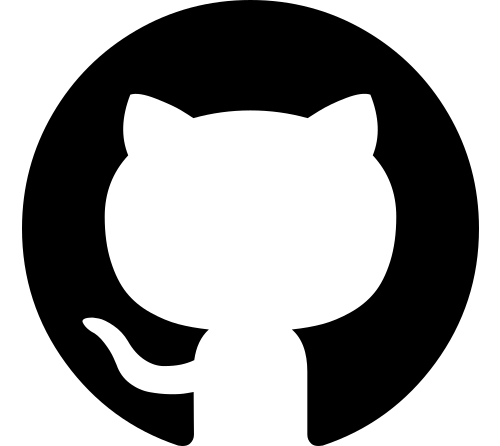
\includegraphics[height=.05\textheight]{resources/github-icon.png}}
  \includegraphics[height=.05\textheight]{resources/discord-icon.png} ComicSansMS /
  \href{https://twitter.com/DerGhulbus/}{
\includegraphics[height=.05\textheight]{resources/twitter-icon.png} @DerGhulbus}

\vspace{20pt}

\begin{center}
  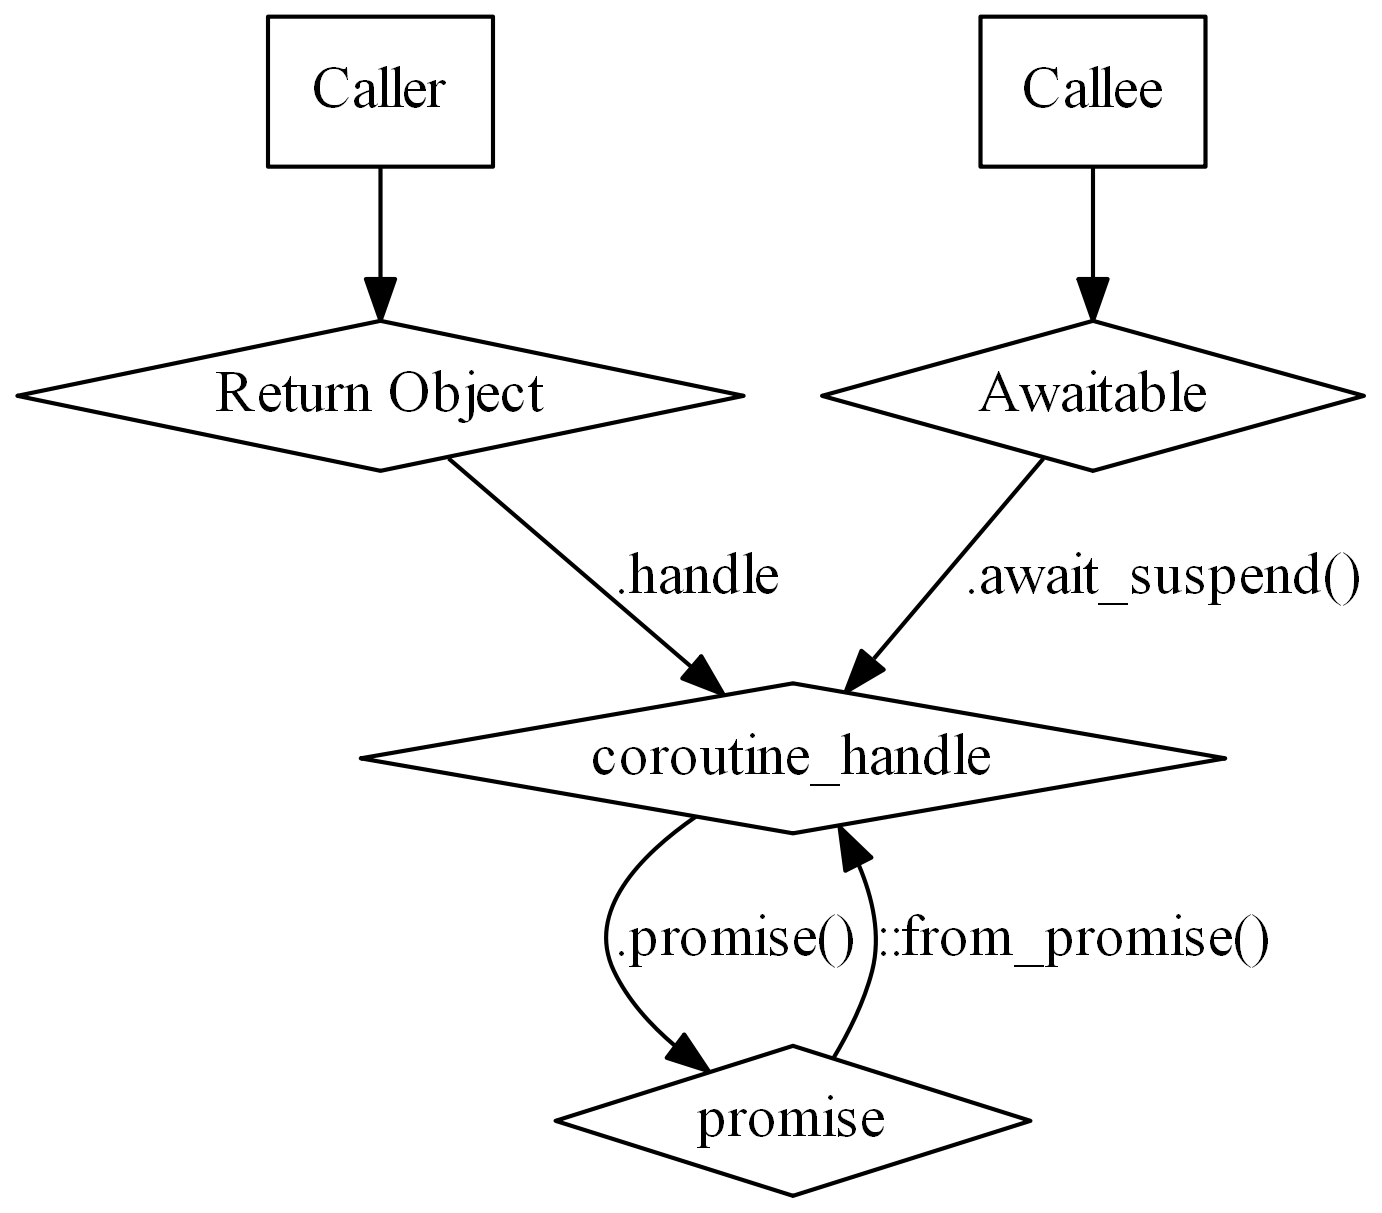
\includegraphics[height=.6\textheight]{pipelinesgfx/acquaintances03.png}
\end{center}

\end{frame}


\end{document}
